\documentclass[10pt,journal,compsoc]{IEEEtran}
\ifCLASSOPTIONcompsoc
  \usepackage[nocompress]{cite}
\else
  \usepackage{cite}
\fi
\ifCLASSINFOpdf
\else
\fi
\usepackage{times}  %Required
\usepackage{helvet}  %Required
\usepackage{courier}  %Required
\usepackage{url}  %Required
\usepackage{graphicx}  %Required
\frenchspacing  %Required
\usepackage{amsmath,amssymb,amsfonts}
\usepackage{algorithmic}
\usepackage{algorithm}
\usepackage{multirow}
\usepackage{makecell}
%\usepackage[boxed]{algorithm2e}
\usepackage{textcomp}
\usepackage{xcolor}
\usepackage{color}
\usepackage{subfigure}
\usepackage{threeparttable}
\usepackage{booktabs}
\usepackage{caption}
\usepackage{tabularx}
\newcommand{\tracy}[1]{\textcolor{purple}{Tracy: #1}}
\def\BibTeX{{\rm B\kern-.05em{\sc i\kern-.025em b}\kern-.08em
		T\kern-.1667em\lower.7ex\hboxd{E}\kern-.125emX}}
\setcounter{secnumdepth}{0}  
\newcommand{\reminder}[1]{\textbf{\color{red}[** #1 **]}}  % to fix
\newcommand{\jt}[1]{\textcolor{red}{[JT: ** #1  **]}}
\newcommand{\jsedit}[1]{\textcolor{blue}{\emph{[JS: #1]}}}
\newcommand{\hide}[1]{} %hide
\newcommand{\vpara}[1]{\vspace{0.06in}\noindent \textbf{#1}}%
\newcommand{\para}[1]{\vspace{0.01in}\noindent\textbf{#1}}%
\newcommand{\secref}[1]{Section~\ref{#1}} %section reference
\newcommand{\Real}{\ensuremath{\mathbb{R}}}  % Real numbers
\newcommand{\figref}[1]{Figure~\ref{#1}} %section reference
\newcommand{\beq}[1]{\vspace{-0.02in}\begin{equation}#1\end{equation}\vspace{-0.02in}}
\newcommand{\beqn}[1]{\vspace{-0.03in}\begin{eqnarray}#1\end{eqnarray}\vspace{-0.03in}}
\newcommand{\beal}[1]{\vspace{-0.03in}\begin{align}#1\end{align}\vspace{-0.03in}}
\newcommand{\besp}[1]{\begin{split}#1\end{split}}
\newcommand{\modelname}[0]{CFIN}
\hyphenation{op-tical net-works semi-conduc-tor}

\begin{document}
\title{Understanding Dropouts in MOOCs}
\author{Wenzheng Feng,\textsuperscript{$\dagger$} Jie Tang\textsuperscript{$\dagger$} \and Tracy Xiao Liu\textsuperscript{$\ddagger$} \\ 
	\textsuperscript{$\dagger$}Department of Computer Science and Technology, Tsinghua University \\
\textsuperscript{$\ddagger$}Department of Economics, School of Economics and Management, Tsinghua University\\
fwz17@mails.tsinghua.edu.cn, jietang@tsinghua.edu.cn, liuxiao@sem.tsinghua.edu.cn

\IEEEcompsocitemizethanks{\IEEEcompsocthanksitem M. Shell was with the Department
of Electrical and Computer Engineering, Georgia Institute of Technology, Atlanta,
GA, 30332.\protect\\
E-mail: see http://www.michaelshell.org/contact.html
\IEEEcompsocthanksitem J. Doe and J. Doe are with Anonymous University.}% <-this % stops an unwanted space
\thanks{Manuscript received April 19, 2005; revised August 26, 2015.}}

\markboth{Journal of \LaTeX\ Class Files,~Vol.~14, No.~8, August~2015}%
{Shell \MakeLowercase{\textit{et al.}}: Bare Demo of IEEEtran.cls for Computer Society Journals}

\IEEEtitleabstractindextext{%
\begin{abstract}
Massive open online courses (MOOCs) have developed rapidly in recent years, and have attracted millions of online users.
However, a central challenge is the extremely high dropout rate --- recent reports show that the completion rate in MOOCs is below 5\%~\cite{onah2014dropout,Kizilcec:2013:DDA:2460296.2460330,Seaton2014Who}. What are the major factors that cause the users to drop out? What are the major motivations for the users to study in MOOCs? In this paper, employing a  dataset from XuetangX\footnote{https://xuetangx.com}, one of the largest MOOCs in China, we conduct a systematical study for the dropout problem in MOOCs. 
We found that the users' learning behavior can be clustered into several distinct categories.
Our statistics also reveal high \textit{correlation} between dropouts of different courses and strong \textit{influence} between friends' dropout behaviors. Based on the gained insights, we propose a Context-aware Feature Interaction Network (CFIN) to model and to predict users' dropout behavior. CFIN utilizes context-smoothing technique to smooth feature values with different context, and use attention mechanism to combine user and course information into the modeling framework. Experiments on two large datasets show that the proposed method achieves better performance than several state-of-the-art methods. The proposed method model has been deployed on a real system to help improve user retention.
%\modelname{} utilizes a feature context-smoothing technique to deal with the sparsity problem, and use the attention mechanisms to combine user and course-specific information into the modeling framework.
%, by incorporating context information in MOOCs. The proposed method achieves state-of-art performance on both KDDCUP open dataset and XuetangX large-scale dataset. Moreover, the framework has been deployed on XuetangX to help users retention.


%Massive open online courses (MOOCs) have developed rapidly in recent years, and have attracted millions of users to receive education online. However, a central challenge is the high dropout rate  for MOOCs learners. Therefore, it is important to understand why users drop out and to predict which users would drop out.

%This paper aims to tackle these two questions. First, we conduct in-depth analyses to identify factors which influence dropout, and propose an effective cluster method to understand users' different engagement pattern. Then we design a series of novel methods to learn behavior features from log data and to learn individual preference based on user-course enrollment graph. Finally, we adopt a unified co-training framework to combine all features. This algorithm allows each model to learn from each other by making use of unlabeled data, which enhances the performance of personalized prediction. The proposed method achieves a state-of-art performance on KDDCUP open dataset, and the system has been deployed on XuetangX\footnote{https://xuetangx.com}  platform.


	

 \end{abstract}


% Note that keywords are not normally used for peerreview papers.
\begin{IEEEkeywords}
Computer Society, IEEE, IEEEtran, journal, \LaTeX, paper, template.
\end{IEEEkeywords}}


% make the title area

	\maketitle
	\section{Introduction}
\begin{figure*}[h]
	\centering
	\subfigure[Age]{
		\centering
		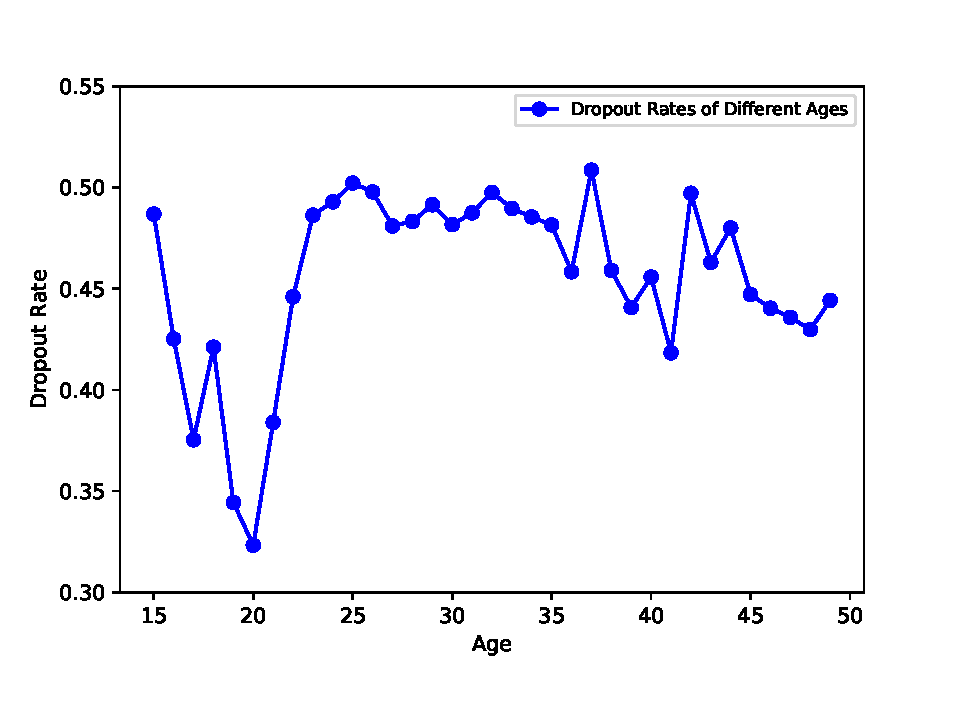
\includegraphics[height=1.69in]{age_dropout.pdf}}%
	\subfigure[Course Category]{
		\centering
		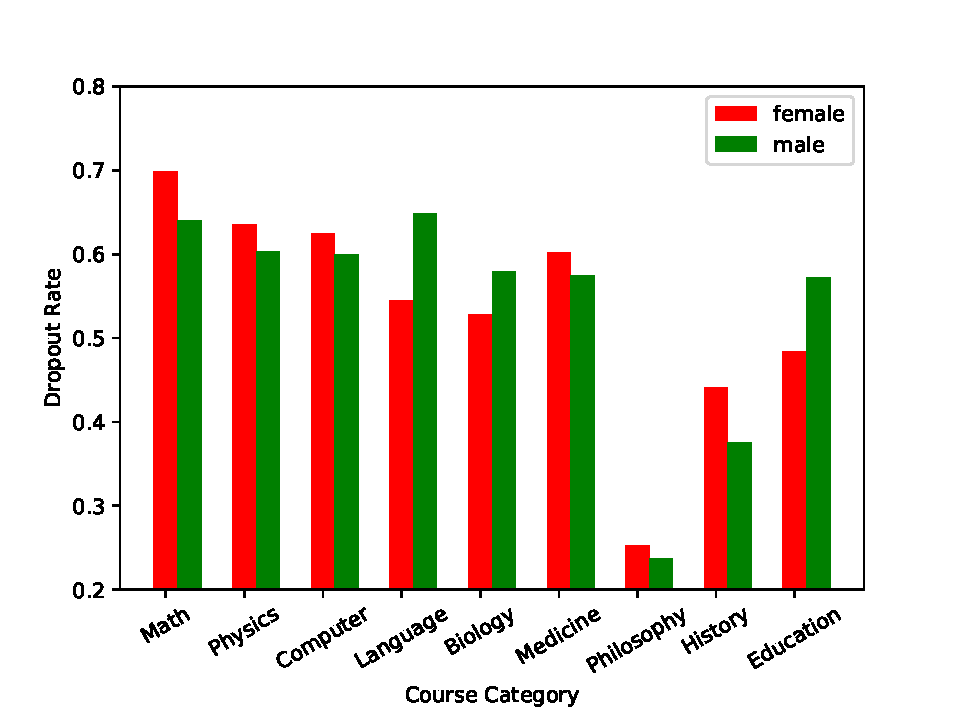
\includegraphics[height=1.7in]{gender_category_prune_2.pdf}
	}
	\subfigure[Education Level]{
		\centering
		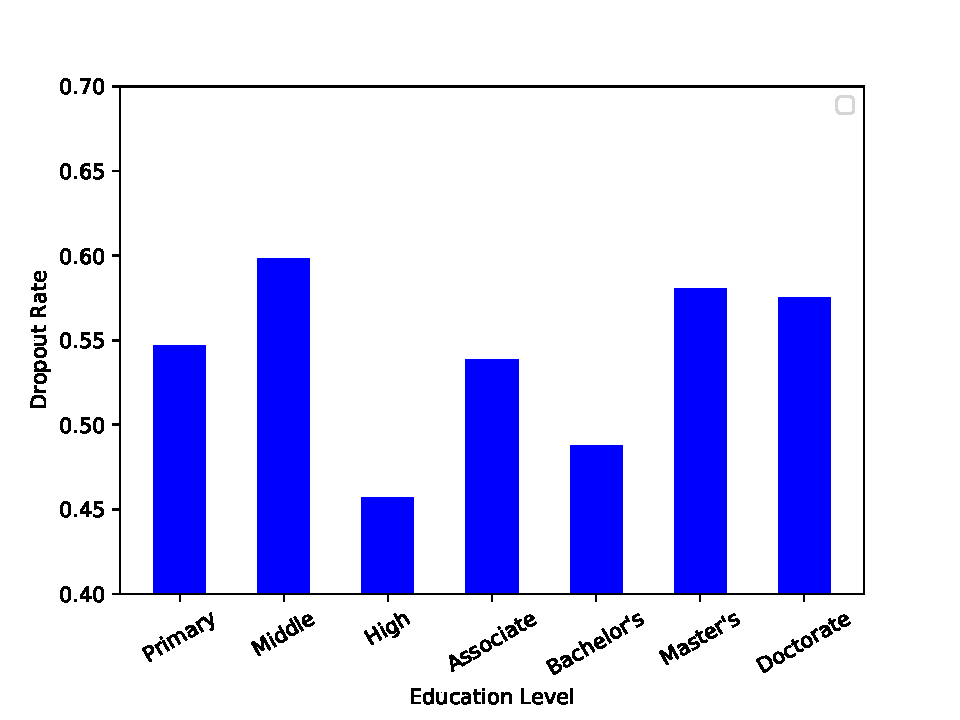
\includegraphics[height=1.7in]{education_stat_prune.pdf}
	}
	%\vspace{-0.1in}
	\caption{Dropout rates of different demographics of users. (a) user age (b) course category (c) user education level.}%. $Y$-axis: dropout rate of users} 
	\label{fig:dropStat} %% label for entire figure 
\end{figure*}

%As a new type of education method, m
% since it appeared in 2012 
%. 
%and XuetangX in China. 
%from more than 800 universities~\cite{shah2018product}. 
Massive open online courses (MOOCs) have become increasingly
popular.
Many MOOC platforms have been launched. For example, Coursera, edX, and Udacity are three pioneers, followed by many others from different countries such as 
XuetangX in China, Khan Academy in North America, Miriada in
Spain, Iversity in German, FutureLearn in England, Open2Study
in Australia, Fun in France, Veduca in Brazil, and Schoo in Japan~\cite{Qiu:2016:MPL:2835776.2835842}.
By the end of 2017, the MOOC platforms have offered 9,400 courses worldwide and attracted 81,000,000 online registered students~\cite{shah2018product}. 
Recently, a survey from Coursera shows that MOOCs are really beneficial to the learners who \textit{complete} courses, where 61\% of survey respondents report MOOCs' education benefits and 72\% of those report career benefits~\cite{zhenghao2015s}. 
%: 61\% of  report MOOCs' educational benefits and 72\% feed back that MOOCs boost their careers. 
%Many MOOCs platforms have been launched up to now, such as Coursera, edX, Udacity, and XuetangX in China.
%Apart from overturning the traditional model of higher education,

However, on the other hand, MOOCs are criticized for the low completion ratio~\cite{He:2015:IAS:2886521.2886563}. 
Indeed, the average course completion rate on edX is only 5\%~\cite{Kizilcec:2013:DDA:2460296.2460330,Seaton2014Who}.
We did a similar statistic for 1,000 courses on XuetangX, and resulted in a similar number --- 4.5\%.
% we find that nearly 79\% users drop out from their enrolled courses. 
\hide{
Meanwhile, the success of MOOCs greatly promote scientific research on education \cite{article,Crow2013}. One of the most urgent research topics is dropout prediction in MOOCs \cite{He:2015:IAS:2886521.2886563}, because of the substantially higher dropout rates on MOOCs than that of traditional education\cite{Clow:2013:MFP:2460296.2460332}, e.g. the average course completion rate on Edx is only 5\% \cite{Kizilcec:2013:DDA:2460296.2460330,Seaton2014Who} and using statistics from over 1000 courses on XuetangX, we find that nearly 79\% users drop out from their enrolled courses. 
}
%Some people argue that the main possible reason for the high dropout rate on MOOCs might be the low monetary cost, i.e., most MOOCs courses are free.
%Some other people state that motivations of the users to study online very differently.
Figure \ref{fig:dropStat} shows several observational analyses. As can be seen, Age is an important factor --- young people are more inclined to drop out; Gender is another important factor --- roughly, female users are more likely to drop science courses and male users are more likely to give up non-science courses; finally, educational background is also important. 
This raises several interesting questions: 1) what are the major dropout reasons? 2) what are the deep motivations that drive the users to study or induce them to drop out?
3) is that possible to  predict users' dropout behavior in advance, so that the MOOCs platform could deliver some kind of useful  interventions~\cite{halawa2014dropout,Qi:18NIPS}?

%, and social pressure for dropping out a course is limited as most MOOCs users take the course online by themselves, while in the traditional classroom setting, students suffer from social pressure when they drop out a course. Therefore, identifying users who have risk of dropout and taking efficient interventions to hold back them is really necessary for MOOC platforms. 
%Furthermore, analyzing individual learning behavior and predicting their likelihood of dropout in a real-time dynamic way can also enhance students learning on MOOCs\cite{halawa2014dropout}. 

%This can help  In the short-run, this can help help instructors to identify users that are in need of scaffolding, and to deliver interventions to help them. In the long term, dropout prediction and analysis can provide valuable insights into the interactions between course design and student factors.  

%dropout analysis and prediction in MOOCs are extremely significant, which would offer both short-term and long-term value\cite{halawa2014dropout}: In the short term, predicting dropout can help instructors to identify users that are in need of scaffolding, and to deliver interventions to help them. In the long term, dropout prediction and analysis can provide valuable insights into the interactions between course design and student factors.
\hide{
In this paper, we focus on studying users' dropout behavior in MOOCs. More specifically, we aims to answer three questions: How to identify dropout reasons of users? How to predict who or when drops out? How to retain users with high risk of dropout in a course? Though several related work, such as user engagement analysis \cite{Anderson:2014:EMO:2566486.2568042ß}, learning behavior prediction\cite{Qiu:2016:MPL:2835776.2835842} and dropout prediction \cite{Nagrecha:2017:MDP:3041021.3054162}, few researches have explored above questions systematically for large scale MOOC learners.

The main challenge to solve theses questions is the diversity of students in MOOCs. Since MOOCs are accessible towards anyone around the world, students in MOOCs have much more diverse background(such as age, education level, location and so on) than those in the traditional classroom. Consequently, their engagement and learning behavior exhibit much more heterogeneity, which further causes different trends of dropout. Our preliminary studies(in Figure \ref{fig:dropStat}) show that different demographics of users in XuetangX exhibits quite different level of dropout rates. However, the data which enable us to learn individual preference for a specific type of users is quite sparse, which causes the difficulty of understanding their dropout motivation and training a personalized dropout prediction model.
}

%In this paper, e%By employing XuetangX, one of the largest Chinese MOOC platforms, as our research source, we 
Employing a  dataset from XuetangX, the largest MOOC platform in China, we aim to conduct a systematical exploration for the aforementioned questions. 
We first perform a clustering analysis over users' learning activity data and found that  users' studying behavior can be grouped into several categories, which implicitly correspond to different motivations that users study MOOC courses.
The analyses also disclose several interesting patterns. 
For example, the dropout rates between similar courses is highly correlated;
friends' dropout behaviors strongly influence each other ---
the probability that a user drops out from a course increases quickly to 65\% when the number of her/his dropout friends increases to 5.

%monotonically from 0.33 to 0.87 when their dropout friends increases from 0 to 10.

\hide{
We first propose a simple but effective method to cluster users based on their temporal engagement patterns, which helps understand users' complex engagement patterns on MOOCs. Furthermore, we conduct statistical analyses to identify potential factors(including co-learning courses and dropout friends(co-learning users))  that affect users' dropout. We have several useful discoveries in this stage. First, we observe that students with lower dropout rate always exhibit higher learning efficiency on course contents and higher correct ratio on homework. Second, dropping out from a course has a positive and significant correlation with dropping out from other co-learning courses. Third, dropout friends indeed have an important influence on users' dropout. The probability that users drop out from their courses increases monotonically from 0.33 to 0.87 when their dropout friends increases from 0 to 10.
}
%Context-aware Feature Interaction Network (CFIN) to 
Based on the analyses results, 
we propose a Context-aware Feature Interaction Network (\modelname{}) to
model and to predict users' dropout behavior. 
In \modelname{}, we utilize a context-smoothing technique to 
smooth values of activity features  using the convolutional neural network (CNN).
%to fuse the information learned from different sources.
Attention mechanisms are then used to combine user and course 
information into the modeling framework.
We evaluate the proposed \modelname{} on two datasets: KDDCUP and XuetangX. The first dataset was used in KDDCUP 2015 and the second one is larger, extracted from the XuetangX system.
Experiments on both datasets 
show that the proposed method achieves much better performance than several state-of-the-art methods. 
We have deployed the proposed method in XuetangX to help improve user retention.

\hide{we then design an algorithm framework to extract a rich set of effective features to capture both activity features and personalized information for each user. Moreover, we utilize deep learning methods, i.e., LSTM and network embedding, to learn latent features from users' activities and social information, which further improve the prediction performance. To assemble these diverse features, we propose a semi-supervised co-training framework to predict users' dropout. By leveraging unlabeled data, this framework can alleviate the sparsity problem. The method achieves \textbf{90.93\%} AUC score on the dataset provided by KDDCUP 2015, which is comparable to the winner team's methods of this competition. We also conduct offline experiments on the large-scale dataset from XuetangX. Our method achieves \textbf{3.14-3.50}\% AUC improvement compared to basic linear classification methods. Furthermore, our framework has been deployed by XuetangX, and facilitating over 10,000,000 registered users retention. 
}
%Figure ? shows our preliminary study for the dropout rates of users of different profiles in XuetangX.  
%However, the information which enables us to identify a particular MOOCs user's background is very limited, which causes the difficulty of understanding her motivation for dropout. 
%Unlike the traditional classroom, MOOCs are accessible towards anyone around the world. Thus MOOCs students have more diverse background. 
%Despite of the importance of predicting dropout rate, it remains substantial difficulty to execute this task accurately. 
%Why, who and when drops out?

%\begin{itemize}
%	\item Since MOOCs are accessible towards anyone around the world, MOOCs students have much more diverse background than those in the traditional classroom. Consequently, their engagement and learning behavior exhibit much more heterogeneity, which further causes different level of dropout rate. However, the information which enables us to identify a particular MOOCs user's background is very limited, which causes the difficulty of understanding her motivation for dropout. 
    %This results in the diverse causes of dropout furthermore. 
   % For an individual user, we don't know who he is and why he comes or drops from MOOCs.
 %   \item  Our analyses show that about 68\% users only enroll in one course on XuetangX. Thus, both the enrollment and log data for a specific user can be rather sparse, and this leads to insufficient training data to learn a user's individual information and to predict her dropout likelihood.
%    \item Since there are numerous underlying factors that are related to a user's dropout behavior on MOOCs, such as user demographics, course categories, and social factors, it is difficult to incorporate all these factors into one unified model for dropout prediction. 
%\end{itemize}


	%We address these challenges as follows. 
%	\textbf{First}, we conduct statistical analyses to identify potential causes that affect users' dropout, and propose a simple but effective method to cluster users based on their temporal engagement patterns, which helps understand users' complex engagement patterns on MOOCs. 
%	\textbf{Second}, based on aforementioned analyses results, we design an algorithm framework to extract a rich set of effective features to capture both activity features and individual information for each user. Moreover, we utilize deeplearning methods, i.e., LSTM and network embedding, to learn latent features from users' activities and user enrollment information, which further improve the prediction performance.
%	 \textbf{Last but not least}, we propose a semi-supervised co-training framework to predict users' dropout via combining these diverse features. By leveraging unlabeled data, this framework can alleviate the sparsity problem.
	




    \section{Related Work}
%\subsection

%\vpara{Dropout Prediction.}
%\textit{Methods used in prior studies} 
%predict student dropout using features extracted from user log, 
  Prior studies apply generalized linear models (including logistic regression and linear SVMs~\cite{Kloft2014,He:2015:IAS:2886521.2886563}) to predict dropout. Balakrishnan et al.~\cite{balakrishnan2013predicting} present a hybrid model which combines Hidden Markov Models (HMM) and logistic regression  to predict student retention on a single course. Another attempt by Xing et al.~\cite{xing2016temporal} uses an ensemble stacking generalization approach to build robust and accurate prediction models.
%rather than directly applying base models. 
Deep learning methods are also used for predicting dropout. For example, Fei et al.~\cite{Fei2015} tackle this problem from a sequence labeling perspective and apply an RNN based model to predict students' dropout probability. Wang et al.~\cite{wang2017deep} propose a hybrid deep neural network dropout prediction model by combining the CNN and RNN.
	Ramesh et al.~\cite{Ramesh:2014:LLE:2893873.2894071} develop a probabilistic soft logic (PSL) framework to predict user retention by modeling student engagement types using latent variables. Cristeaet et al.~\cite{cristea2018earliest} propose a light-weight method which can predict dropout before user start learning only based on her/his registration date.
Besides prediction itself, Nagrecha et al.~\cite{Nagrecha:2017:MDP:3041021.3054162}  focus on the interpretability of existing  dropout prediction methods. Whitehill et al.~\cite{whitehill2015beyond} design an online intervention strategy to boost users' call-back in MOOCs. Dalipi et al.~\cite{dalipi2018mooc} review the techniques of dropout prediction and propose several insightful suggestions for this task. What's more, XuetangX has organized the KDDCUP 2015\footnote{https://biendata.com/competition/kddcup2015} for dropout prediction. In that competition, most teams adopt assembling strategies to improve the prediction performance, and ``Intercontinental Ensemble'' team get the best performance by assembling over sixty single models.
%The authors explore each stage of the prediction pipeline %and propose some insights of why a 
	 
     
%\subsection
%\vpara{Engagement Pattern Mining.} 
More recent works mainly focus on analyzing students engagement based on statistical methods and 
%some of them 
explore how to improve student engagements~\cite{kellogg2013online,reich2015rebooting}. 
\hide{
Kizilcec et al.~\cite{Kizilcec:2013:DDA:2460296.2460330} employ a cluster method to identify the longitudinal engagement trajectories. Anderson et al.~\cite{Anderson:2014:EMO:2566486.2568042ß} provide a taxonomy for student engagement patterns and study the relationship between student grades and their engagement. Guo et al.~\cite{Guo:2014:VPA:2556325.2566239} analyze how student engagement pattern varies with different video types. Kim et al.~\cite{Kim:2014:UID:2556325.2566237} discover high dropout rate often occurs in long videos, and students who re-watch videos are more likely to drop out than  first-time watchers. }%
Zheng et al.~\cite{Zheng:2015:USM:2675133.2675217} apply the grounded theory  to study users' motivations for choosing a course
%, their learning perceptions and engagement patterns, and 
and to understand 
%underlying 
the reasons that users drop out a course. Qiu et al.~\cite{Qiu:2016:MPL:2835776.2835842} study the relationship between student engagement and their certificate rate, and propose a latent dynamic factor graph (LadFG) to model and predict learning behavior in MOOCs. 
\hide{
Chaturvedi et al.~\cite{chaturvedi2014predicting} propose a framework to predict instructor's intervention on forums. 
Ramesh et al.~\cite{ramesh2015weakly} develop a weakly supervised joint model for aspect-sentiment analysis in forums. 
Maximilian et al.~\cite{He:2016:MMM:3015812.3015989} use topic models for the psychometric testing of MOOC students based on their forum activities. 
Utilizing data from a Coursera class, Yang et al.~\cite{yang2013turn} use a survival model to measure the impact of certain factors on dropout rate.
Some other related study could be also found in~\cite{bayer2012predicting}.
, e.g., factors related to student behavior and social positioning within discussion forums. Other social behavior, such as email and discussion board conversation, is also shown as effective factors for predicting dropout \cite{bayer2012predicting}.
}

%\subsection{Co-training}
	%As a most efficient semi-supervised method, co-training framework is introduced by Blum and Mitchel in \cite{Blum:1998:CLU:279943.279962}. With training multiple learners for one task, the unlabeled samples are utilized to augment training set for each leaner. Following this idea, a number of studies emerge to explore the potentials of co-training. For example,  Nigam et al. \cite{Nigam:2000:AEA:354756.354805} performed extensive experiments for comparing the performance of co-training and other popular semi-supervised algorithm, EM-algorithm\cite{10.2307/2984875}. And the experiments showed that co-training outperforms EM even on tasks where there is no natural split of features.Zhou et al. \cite{Zhou:2005:SRC:1642293.1642439} has proposed a novel co-training style regression algorithm, this algorithm used two $k$-nearest neighbor regressors with different distance metrics, and experiments show that it can effectively exploit unlabeled data to improve regression estimates. In \cite{Zhang:2014:ACS:2600428.2609599}, co-training algorithm was applied to address the cold-start problem in recommender systems, authors combined the factorization model co-training algorithm to capture fine-grained user-item context. 
	%the experiments on real-word datasets show that the recommendation accuracy is significantly improved compared to standard algorithms and the cold-start problem is largely alleviated.
	
%	\section{PRELIMINARY}
\begin{table}
	\centering
	\caption{The Description for User Activities on XuetangX.}
	\setlength{\tabcolsep}{2mm}{
	\begin{tabular}{c|c|c}
		\hline \hline
		Resource & Action & Description \\
		\hline
		\multirow{3}{*}{video}& watch & play and watch video \\
		\cline{2-3}
		& stop & pause video or watching video over\\
		\cline{2-3}
		& jump& jump to another position of video\\
		\hline
		\multirow{2}{*}{forum}& question & publish a question on forum \\
		
		\cline{2-3}
		& answer & answer a question  on forum  \\
		\hline
		\multirow{3}{*}{assignment}& correct & submit a correct answer\\
		\cline{2-3}
		&wrong  & submit a wrong answer\\
		\cline{2-3}
		& reset & revise and resubmit an answer\\
		\hline
		\multirow{2}{*}{web page} &access & access a page in course \\
		\cline{2-3}
		& close  & close a page in course \\ 
		\hline \hline
	\end{tabular}}
	\label{ResourceAction}
\end{table}

\subsection{Problem Formulation}
		\label{ProblemDef}
		    \begin{figure}
			\centering
			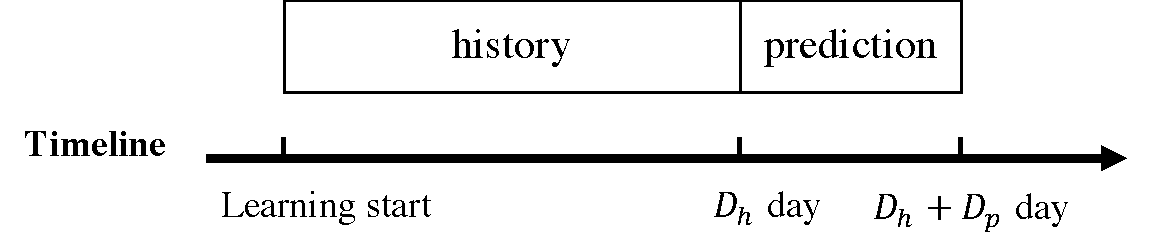
\includegraphics[width=\linewidth]{course-span.pdf}
			
			\caption{Dropout Prediction Problem. The first $D_h$ days are \emph{history period}, and the next $D_p$ days are \emph{prediction period}.}
			\label{fig:dataCons}
		\end{figure}
	Our main task is to predict whether a user would dropout from an enrolled course in a pre-specified time window. In order to formulate this problem, we introduce the following definitions. \\


	\emph{Definition 1.} \textbf{Enrollment Relation}: Let $\mathbb{C}$ denote the set of courses, and $\mathbb{U}$ denote the set of users. 
	The set of enrolled courses of $u\in \mathbb{U}$ is denoted by $\mathbb{C}_u\subset \mathbb{C}$, ($c\in\mathbb{C})$.  $\mathbb{U}_c\subset \mathbb{U}$ refers to the set of users who have enrolled in $c$. Then the set of enrollment relations is defined as $\mathbb{E}=\{(u,c)|u\in \mathbb{U}, c\in \mathbb{C}_u\}$.\\
	
    
	\emph{Definition 2.} \textbf{Learning Activity}: 
	In MOOCs, user's learning activity can be formulated into a paired tuple  $x = (a, t)$, where $a$ represents user's action(such as ``watching video'') and $t$ is the corresponding logged time stamp. In this paper, we focus on four types of learning activities: \emph{video, forum, assignment, web page}, which are described in table \ref{ResourceAction}. \\
	
	%Each course has a set of available resources for users, such as video and forum. 
	%Here we use $R$ to represent the resource set of course on MOOCs. For each resource $r \in R$, there are a set of specific actions for it. We use $A$ to denote the action set. In this paper, we focus on four types of resources on MOOCs: \emph{video, forum, assignment, web page}, which are shown in table \ref{ResourceAction}, together with the corresponding actions. 
    
    %Then a learning activity record of $u\in \mathbb{U}$ in one enrolled course $c\in \mathbb{U}_c$ at time $t$ can be represented as $X=(u,c,r,a,t)$, where $r\in R$ is the resource $u$ has accessed, $a\in A$ is the corresponding action on $r$. For each $(u,c) \in \mathbb{E}$, we use $\mathcal{X}_{uc}$ to represent user $u$'s historical learning activity set on $c$.\\
	
	
    \emph{Definition 3.} \textbf{Dropout Prediction}: Given user $u$'s activity sequence $X_{(u,c)}= [x_1, x_2,...,x_N]$ on course $c$ in \textit{history period}(as shown in Figure \ref{fig:dataCons}, it is the first $D_h$ days after the learning starting time), our goal is to predict whether $u$ will drop out from $c$ in the \textit{prediction period}(as shown in Figure \ref{fig:dataCons}, it is the following $D_p$ days after \textit{history period}). More precisely, let $y_{(u,c)} \in \{0,1\}$ denote the ground truth of whether $u$ has dropped out, $y_{(u,c)}$ is positive if and only if $u$ has not taken activities on $c$ in the \textit{prediction period}. Then our task is to learn a function:
	 $$f: (u,c,X_{(u,c)})\to y_{(u,c)}$$
     
\subsection{XuetangX platform}

	XuetangX is one of the largest MOOCs platforms in China, which was launched in October 2013. It has provided over 1000 courses and attracted more than 10,000,000 registered users up to now.  XuetangX type courses into twelve categories based on their learning objects: \textit{art, biology, computer science, economics, engineering, foreign language, history, literature, math, philosophy, physics,} and \textit{social science}. Moreover, users can take two types of courses: \textit{Instructor-paced mode }and \textit{Self-paced mode.} An Instructor-paced mode course follows the same class schedule as offline courses, while a Self-paced one has more flexible schedule and students can arrange their learning time at any of their convenient time.
	%\textbf{Instructor-Paced} courses progress at the pace that the course author sets. In these courses, students cannot access course content before its release date, and learners must complete assignments by their due dates. \\
	%\textbf{Self-Paced} courses are another kind of courses. Different from Instructor-Paced courses, Self-Paced courses give students much more freedom, where they can access all course materials when the course begins, and assignments do not have due dates. \\ 
	Our dataset includes both Instructor-paced  and Self-paced courses. We utilize two datasets in our experiments: a smaller dataset from KDDCUP (named as \textit{``KDDCUP dataset"}) and a much larger dataset from XuetangX (named as \textit{``XuetangX Large-Scale Dataset"}). Our dataset includes historical user log, user-level course enrollment, user demographics and course related information. We describe these two datasets in more details below:
    
	 \noindent\textbf{KDDCUP Dataset.}
	KDDCUP 2015\footnote{https://biendata.com/competition/kddcup2015/} is one of the most heated competitions which aims to predict students' dropout on XuetangX, and has attracted 821 teams to participate. In that competition, participates need to predict the whether a user will drop a course within next 10 days based on her historical activities in prior 30 days, i.e., ($D_h=30$, $D_p$=10). 
	 This data is relatively limited as it only covers 39 Instructor-paced courses and does not contain some important information, such as user demographics and course categories.
	 %Table \ref{tab:KDDdata} reports the descriptive statistics of this dataset. 
	
	\noindent \textbf{XuetangX Large-Scale Dataset.}
 	After KDDCUP 2015, XuetangX launched many more courses and attracted millions of users. 
    %In order to avoid the limited scale of data, 
To make our methods more robust and generalizable, we further construct a much larger and richer dataset than KDDCUP dataset. This dataset contains 698 Instructor-paced courses and 515 Self-paced courses. To identify a optimal time span for the history period and prediction period, we test the variety of prediction performance when selecting different values for $D_h$ and $D_p$. And we can observe that prediction results become better as $D_h$ gets larger and $D_p$ gets smaller. Considering the model's efficiency and applicability trade-off, we final adopt the following strategy: For instructor-paced courses, $D_h=35$, $D_p=10$. While for self-paced courses, $D_h=60$, $D_p=10$. Since learners’ behaviors
in Self-paced courses exhibit more heterogeneity, the larger
choice of $D_h$’s value for Self-paced courses is to make the
training data more sufficient.
%Table \ref{tab:XuetangXdata} reports the corresponding summary statistics.\\
	



    



\section{Data and Insights}
%\subsection{Data}

The analysis in this work is performed on two datasets from XuetangX.
XuetangX, launched in October 2013, is now one of the largest MOOC platforms in China.
%, which was launched in October 2013. 
It has provided over 1,000 courses and attracted more than 10,000,000 registered users.
% up to now.  
XuetangX has twelve categories of courses: art, biology, computer science, economics, engineering, foreign language, history, literature, math, philosophy, physics, and social science. 
%Moreover, 
Users in XuetangX can choose the learning mode: Instructor-paced Mode (IPM) and {Self-paced Mode (SPM)}.  IPM   follows the same course schedule as conventional classrooms, while in SPM, one could have more flexible schedule to study online by herself/himself. Usually an IPM course spans over 16 weeks in XuetangX, while an SPM course spans a longer period.
Each user can enroll one or more courses. When one studying a course, the system records multiple types of activities: video watching (watch, stop, and jump), forum discussion (ask questions and replies), assignment completion (with correct/incorrect answers, and reset), and web page clicking (click and close a course page).

\vpara{Two Datasets.}
%We use two datasets in this study. Both are from XuetangX.
%Our dataset includes both Instructor-paced  and Self-paced courses. We utilize two datasets in our experiments: 
The first dataset contains 39 IPM  courses and their enrolled students. It
was also used for KDDCUP 2015. Table~\ref{tab:KDDdata} lists   statistics of this dataset. With this dataset, we compare our proposed method with existing methods, as the challenge has attracted 821 teams to participate.
We refer to this dataset as KDDCUP.

The other dataset contains 698 IPM courses and 515 SPM courses. Table~\ref{tab:XuetangXdata} lists  the statistics. The dataset contains richer information, which can be used to test the robustness and generalization of the proposed method.
This dataset is referred to as XuetangX.



\begin{table}
	\centering
	\caption{Statistics of the KDDCUP dataset.}
\small
	\setlength{\tabcolsep}{3mm}{\begin{tabular}{l|l|r}
			\hline \hline
			
			Category&  Type   & Number\\
			\hline
			\multirow{3}{*}{log} & \# video activities & 1,319,032\\
			
			&  \# forum activities & 10,763,225\\
			
			& \# assignment activities & 2,089,933 \\
			
			& \# web page activities & 738,0344 \\
			\hline
			\multirow{5}{*}{enrollment} &  \# total &  200,904  \\
			
			& \# dropouts & 159,223 \\
			
			& \# completions &41,681 \\
			
			& \# users &  112,448   \\
			
			&  \# courses &    39   \\	
			\hline \hline
	\end{tabular}}
	\label{tab:KDDdata}
	\normalsize
\end{table}
\begin{table}
	\centering
	\caption{Statistics of the XuetangX dataset.}
	\small
	\begin{threeparttable}
		\setlength{\tabcolsep}{1.3mm}{\begin{tabular}{l|l|r|r}
				\hline \hline
				Category & Type   &\#IPM\tnote{*}  & \#SPM\tnote{*} \\
				\hline
				\multirow{3}{*}{log} &\# video activities & 50,678,849&  38,225,417 \\
				
				& \# forum activities & 443,554 &   90,815\\
				
				&  \# assignment activities & 7,773,245& 3,139,558 \\
				
				& \# web page activities   & 9,231,061 & 5,496,287\\
				\hline
				\multirow{5}{*}{enrollment} &  \# total  & 467,113 & 218,274\\
				
				& \# dropouts &372,088 & 205,988\\
				
				&  \# completions  & 95,025 & 12,286\\
				
				& \#  users   &254,518 & 123,719\\
				
				& \# courses   & 698& 515\\	
				\hline \hline
		\end{tabular}}
			\begin{tablenotes}
			\footnotesize
			\item[*] \#IPM and \#SPM respectively stands for the number for the corresponding IPM courses and SPM courses.%, and  represents the number of SPM courses.
		\end{tablenotes}
	\end{threeparttable}
	\label{tab:XuetangXdata}
	\normalsize
\end{table}


%\section{Observational Analysis}
%	\label{sec:analysis}
    %\subsection{Data Preprocessing}

   % In order to construct the dataset used for training model, we need to manually divide the whole course duration into $history$ period and $future$ period. Figure \ref{fig:dataCons} presents the data construction strategy. We use the first $D_h$ days after the learning starting time as the  $history$ period, while $future$ period is from $D_h+1$-st day to $(D_h+D_f)$-th day. For \textit{KDDCUP dataset} and Instructor-paced courses in \textit{XuetangX Large-Scale Dataset}, the learning starting time is defined as the course starting time, while for Self-paced courses in \textit{XuetangX Large-Scale Dataset}, we treat user's first visiting time to the course as the learning start time. For \textit{KDDCUP dataset}, $D_h$ and $D_f$ are set to $30$ and $10$ respectively by the organizers of \textit{KDDCUP 2015}. As for \textit{XuetangX Large-Scale Dataset}, we adopt different strategies for Instructor-and Self-paced courses. For Instructor-paced courses, we set $D_h=35$, $D_f=10$, while for Self-paced courses $D_h=60, D_f=10$. Since learners' behaviors in Self-paced courses exhibit more heterogeneity, the larger choice of  $D_h$'s value for Self-paced courses is to make the training data more sufficient.  
    
\subsection{Insights} 
    \label{sec:temporal}
     
\hide{
    In order to study users' different engagement patterns on XuetangX, we propose a cluster method by using users ``temporal codes'' as input, which encode a user's activities on courses into a vector. The definition is below.
}
    Before proposing our methodology, we try to gain a better understanding of the users' learning behavior.
    We first perform a clustering analysis on users' learning activities. To construct the input for the clustering analysis, we define a concept of \textit{temporal code} for each user. 
    %Formally, we have
    
    \emph{Definition 1.} \textbf{Temporal Code}:
    For each user $u$ and one of her enrolled course $c$, the temporal code is defined as a binary-valued vector $\mathbf{s}^u_{c}=[s^u_{c,1}, s^u_{c,2},..., s^u_{c,K}]$, where $s^u_{c,k} \in \{0,1\}$ indicates whether user $u$ visits course $c$ in the $k$-th week. Finally, we concatenate all course-related vectors and generate the temporal code for each user 
    as $\mathbf{S}^u=[\mathbf{s}^u_{c_1}, \mathbf{s}^u_{c_2},..., \mathbf{s}^u_{c_M}]$, where $M$ is the number of courses.
    
    Please note that the temporal code is usually very sparse. We feed the sparse representations of all users' temporal codes into a $K$-means algorithm.
    The number of clusters is set to $5$ based on a \textit{Silhouette Analysis}~\cite{rousseeuw1987silhouettes} on the data. 
    Table~\ref{tab:clusterStat} shows the clustering results. It can be  seen that 
    both cluster 2 and cluster 5 have low dropout rates, but more interesting thing is that users of cluster 5 seem to be hard workers --- with the longest video watching time, while users of cluster 2 seem to be active forum users --- the number of questions (or answers) posted by these users is almost $10\times$ higher than the others. This corresponds to different motivations that users come to MOOCs. Some users, e.g., users from cluster 5, use MOOC to seriously study knowledge, while some other users, e.g., cluster 2, may simply want to meet friends with similar interest.
    %    while the dropout rates for users in the other three clusters are much higher. We also find that the dropout probability is significantly correlated with users' activity frequency. For example, users in cluster 2 and 5 have more video activities than users in other three clusters, which indicates users in these two clusters watch more course videos. Although users in clusters 2 and  5 have a similar dropout probability, their engagement patterns are quite different. Comparing to cluster 2, users in cluster 5 have more video activities and less forum activities. This suggests that those in cluster 5 may prefer to studying by themselves, whereas those in cluster 2 are more interested in discussing with other students. 
    Another interesting phenomenon is about users in cluster 4. Their average number of revise answers for assignment (i.e.  \#reset) is much higher than all the other clusters.
    %with high dropout rate, i.e. clusters 1 and 3. 
    Users of this cluster probably are students with difficulties to learn the corresponding courses.
    %This suggests that these users may care more about their grades on MOOCs, and this may lead to the fact that their average dropout rate is lower than users in cluster 1 (0.66 vs 0.78) and cluster 3 (0.66 vs 0.83).  
    
    
    \begin{table}
    \hspace{-0.01in}
    	\centering
    	\caption{Results of clustering analysis. C1-C5 --- Cluster 1 to 5; CAR --- average correct answer ratio. }
    	\small
    	\label{tab:clusterStat}
    	\setlength{\tabcolsep}{1mm}\begin{tabular}{@{}c@{}|l@{}|c|c|c|c|c@{}}
    		\hline
    		\hline
    		Category &  Type   & C1& C2 & C3& C4&C5 \\
    		\hline
    		\multirow{3}{*}{video}&  \#watch &21.83 &46.78 &12.03&19.57 & \textbf{112.1}\\	
    		\cline{2-7}
    		& \#stop     &28.45 & 68.96&20.21&37.19& \textbf{84.15}\\
    		\cline{2-7}
    		& \#jump   &16.30 & 16.58& 11.44& 14.54& \textbf{21.39} \\
    		\hline
    		\multirow{2}{*}{forum}&  \#question & 0.04 & \textbf{0.38} &0.02 & 0.03 & 0.03 \\
    		\cline{2-7}
    		& \#answer &0.13 &\textbf{3.46}&0.13&0.12&0.17\\
    		\hline
    		\multirow{2}{*}{assignment} & CAR &0.22 & \textbf{0.76} & 0.19& 0.20 & 0.59\\
    		\cline{2-7}
    		& \#revise  &0.17 & 0.02& 0.04& \textbf{0.78}& 0.01\\
    		\hline
    		\multirow{2}{*}{session}    & seconds &1,715 &714& \textbf{1,802}& 1,764& 885\\
    		\cline{2-7}                
    		&  count     &3.61 &\textbf{8.13}& 2.18&4.01& 7.78\\ 
    		\hline
    		\multirow{2}{*}{enrollment} & \#enrollment & 21,048 & 9,063&\textbf{401,123} &25,042 & 10,837\\
    		\cline{2-7}
    		& total \#users & 2,735 & 4,131& \textbf{239,302} & 4,229 & 4,121 \\
    		\cline{2-7}
    		& dropout rate &0.78 &0.29 &\textbf{0.83} &0.66 &0.28\\
    		\hline	
    		\hline
    	\end{tabular}
    	\normalsize
    \end{table}

\hide{
    her temporal code  a course $c \in \mathbb{C}$ in the first $K$ weeks is represented as a vector code $\mathbf{s}^u_{c}=[s^u_{c,1}, s^u_{c,2},..., s^u_{c,K}]$, where $s^u_{c,k} \in \{0,1\}, (1 \le k \le K)$ represents whether $u$ visit $c$ in $k$-th week. Note that  $\mathbf{s}^u_{c}$ is set to all $0$ if $u$ has not enrolled in $c$. Then the ``temporal code'' of $u$ is obtained by concatenating all course temporal vectors: $\mathbf{S}^u=[\mathbf{s}^u_{c_1}, \mathbf{s}^u_{c_2},..., \mathbf{s}^u_{c_M}], c_m \in \mathbb{C}, $$(1 \le m \le M)$. \\


    In experiments, we use the first $5$ week logs to construct the ``temporal codes'', i.e. $K=5$. All users' ``temporal codes'' are input to a K-means algorithm for clustering users. Based on the \textit{Silhouette Analysis}, the number of clusters is set to $5$.	The statistics of $5$ clusters are described in Table \ref{tab:clusterStat}. Both clusters 2 and 5 have low dropout rates, while the dropout rates for users in the other three clusters are much higher. We also find that the dropout probability is significantly correlated with users' activity frequency. For example, users in cluster 2 and 5 have more video activities than users in other three clusters, which indicates users in these two clusters watch more course videos. Although users in clusters 2 and  5 have a similar dropout probability, their engagement patterns are quite different. Comparing to cluster 2, users in cluster 5 have more video activities and less forum activities. This suggests that those in cluster 5 may prefer to studying by themselves, whereas those in cluster 2 are more interested in discussing with other students. Another intriguing phenomenon is about users in cluster 4. Their average number of revise answers for assignment (i.e. Avg. \# reset) is much higher than the other 2 clusters with high dropout rate, i.e. clusters 1 and 3. This suggests that these users may care more about their grades on MOOCs, and this may lead to the fact that their average dropout rate is lower than users in cluster 1 (0.66 vs 0.78) and cluster 3 (0.66 vs 0.83).  
}    

    
	%\subsection{Dropout Correlation between Courses}
    
    
    \vpara{Correlation Between Courses.}
    We further study whether there is any correlation for users dropout behavior between different courses. 
    Specifically, we try to answer this question: will someone's dropout for one course increase or decrease the probability that she drops out from another course?
    %user's likelihood of dropping out in other registered courses? and \emph{How does the degree of influence change with time?} 
    %To answer these two questions, 
    We conduct a regression analysis to examine this.
    %across weeks. 
    A user's dropout behavior in a course is encoded as a 16-dim dummy vector, with each element representing whether the user has visited the course in the corresponding week (thus 16 corresponds to the 16 weeks for studying the course). The input and output of the regression model are two dummy vectors which indicate a user's dropout behavior for two different courses in the same semester. By examining the slopes of regression results (Figure~\ref{fig:courseLinreg}), we can observe a significantly positive correlation between users' dropout probabilities of different enrolled courses, 
    %across periods, 
    though overall the correlation decreases over time. 
    Moreover, we did the analysis for courses of the same category and those across different categories. It can be seen that the correlation between courses of the same category is higher than courses from different categories. 
    One potential explanation is that when a user has limited time to study MOOC, they may first give up substitutive courses instead of those with complementary knowledge domain. 
    

%As shown in Figure \ref{fig:courseLinreg} , we could observe that the dropout correlation between courses is significantly positive, i.e., \emph{if user dropout from one course, then he will more likely drop out from another course at the same time,}  and the correlation  \emph{decreases} with the passing of time in a term.  What's more, we could observe that the slopes of experiments on same category courses are larger than those of experiments on different category courses, which means that the dropout influence from same category courses is stronger than the influence from different category courses.
	
	\begin{figure}[t]
	\centering 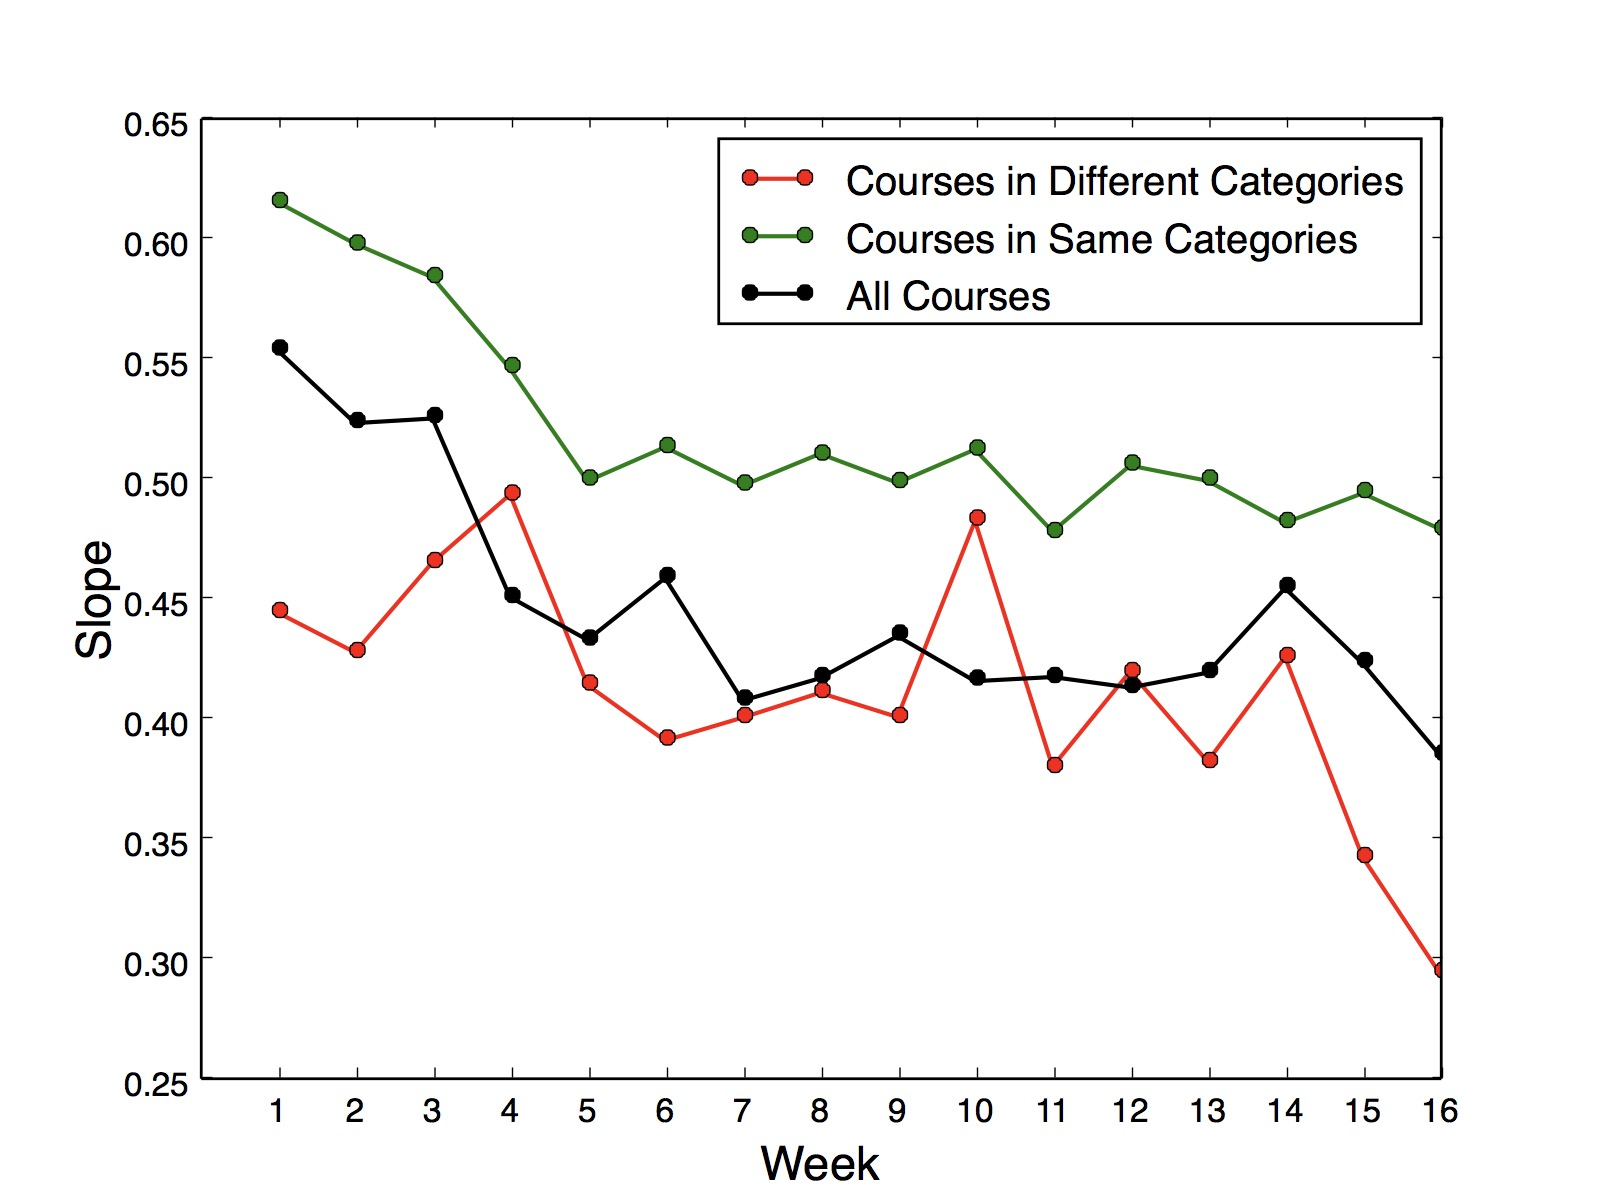
\includegraphics[ height=5cm]{lingress_slope.jpg}
	\caption{Dropout correlation analysis between courses. The $x$-axis denotes the weeks from 1 to 16 and the $y$-axis is the slope of linear regression results for dropout correlation between two different courses. The red line is the result of different category courses, the green line denotes the slope of same category courses, and the black line is pooling results in all courses.}
	\label{fig:courseLinreg}
	\end{figure}
	
	\begin{figure}[t]
	\centering
		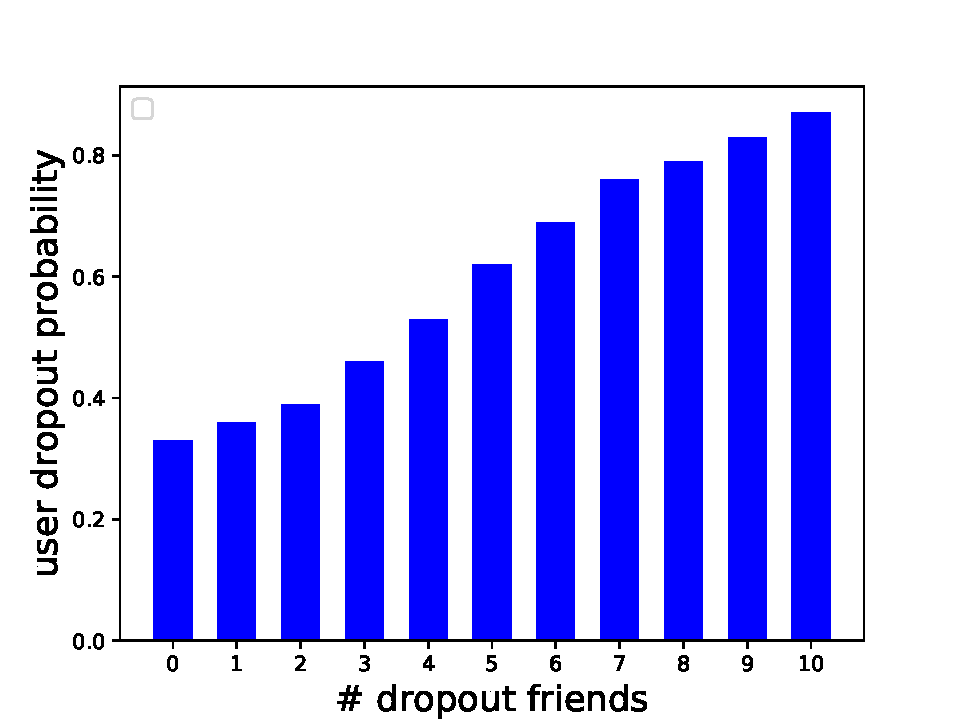
\includegraphics[height=5cm]{friends_inf.pdf}
		\caption{User dropout probability conditioned on the number of dropout friends. $x$-axis is the number of dropout friends, and $y$-axis is user's dropout probability.}
		\label{fig:friendInf}
	\end{figure}
	
	%\subsection{Influence From Dropout Friends}
    
	%\label{sec:influence}
\vpara{Influence From Dropout Friends.}
	%In real life, users' behaviors are easily affected by their friends. 
	Users' online study behavior may influence each other~\cite{Qiu:2016:MPL:2835776.2835842}. We did another analysis to understand how the influence would matter for dropout prediction.
    %In this section, we analyze the 
    %users' dropout behavior would be influenced their friends.
    In XuetangX, the friend relationship is implicitly defined using co-learning relationships. 
    More specifically, 
    %correlation between users and their friends. One bottleneck of this task is that because of the limited social activity data on MOOCs, it is difficult for us to identify the social relationship between users. Therefore, we simply assume that a user's friends are co-learning students who have similar learning interests with her, and 
    we use a network-based method to discover users' friend relationships. First, we build up a user-course bipartite graph $G_{uc} $ based on the enrollment relation.
	 %set $\mathbb{E}$. $G_{uc}$ is a bipartite graph whose 
	 The nodes are all users and courses, and the edge between user $u$ and course $c$ represents that $u$ has enrolled in course $c$. Then we use DeepWalk~\cite{Perozzi:2014:DOL:2623330.2623732}, an algorithm for learning representations of vertices in a graph, to learn a low dimensional vector for each user node and each course node in $G_{uc}$. Based on the user-specific representation vectors, we  compute the cosine similarity between  users who have enrolled a same course. Finally, those users with high similarity score, i.e., greater than 0.8, are considered as friends. 

In order to analyze the influence from dropout friends quantitatively, we calculate users' dropout probabilities conditional on the number of dropout friends.
Figure~\ref{fig:friendInf} presents the results. We see users' dropout probability increases monotonically from $0.33$ to $0.87$ when the number of dropout friends ranges from $1$ to $10$. This  indicates that a user's dropout rate is greatly influenced by her/his friends' dropout behavior.
	 
	
    
    %%co-training version:
	 %\section{Feature Learning}
	
	\label{sec:allFeat}
  Features used in our system are categorized to three types: activity features, user-related features, and course-related features, which are defined as $\mathbf{Feat}_a$, $\mathbf{Feat}_u$ and $\mathbf{Feat}_c$, respectively. Activity features mainly include users' learning behaviors, which are extracted from user historical activity sequence. User- and course-related features are mainly from user-course enrollment graph.
  %and these two sets of features are mainly used to capture user and course information from the perspective of user and course respectively.
  
	%And, in order to capture the context information for MOOC users, a series of user-related features and course-related features are  also used in our framework. 
	\subsection{Activity Features}
	
	\label{sec:activityFeat}
This set of features are from user historical activity logs. We employ both statistical methods and a Long Short-Term Memory (LSTM) framework to learn user behavior patterns. This part of features are represented by $\mathbf{Feat}_{a}$. \\\\
\noindent \textbf{Statistics Features}
\begin{enumerate}
	\item{Activity Count/Ratio:} For each enrollment $(u,c)$, we calculate the number and ratio for each type of activities in table \ref{ResourceAction}. 
	\item{Activity Temporal Statistics:} The whole duration time of a course is divided by weeks, and the activity counts and statistics(including \emph{max, min, stdev, median}) in different weeks are used as features.
	\item{Activity Count in Hours Per Day:} We calculate user activity count for each hour in a day (24 hours).
	\item{Activity Count in Day Per Week:} We compute user activity count for each day in a week (5 weekdays + 2 weekends).
	\item{Activity N-gram Count/Ratio:} The N-grams of activity sequence is used to capture the correlations between neighbor activities. We employ N-gram activity count and ratio as the N-gram features.
	\item{Engagement Style:} Following the taxonomy of engagement introduced by Anderson et al. \cite{Anderson:2014:EMO:2566486.2568042ß}, we use the $\emph{assignment fraction} = \frac{ \emph{watching video \#}}{ \emph{complete assignment \#}}$ to represent user's engagement pattern.
	\item{Learning Time Span:} A user's learning time span is the duration between a user's first visit time and her last visit time on a course.  
	
	\item{Effective Learning Time:} The \emph{effective learning time} introduced by Qiu et al. \cite{Qiu:2016:MPL:2835776.2835842} is an approximated method to compute user's actual study time on a certain course. This is calculated based on the time interval between user's \emph{watching video} and \emph{stop video}, and we employ this feature in our paper.
	
	\item{Visiting Time Interval:} A user's interval time for visiting one course reflects user's interests in this course. The statistics(\emph{max, min, stdev, median}) of visiting time intervals are used as features.\\
\end{enumerate}


\noindent \textbf{LSTM Temporal Features}\\
	\begin{figure}
	\centering
	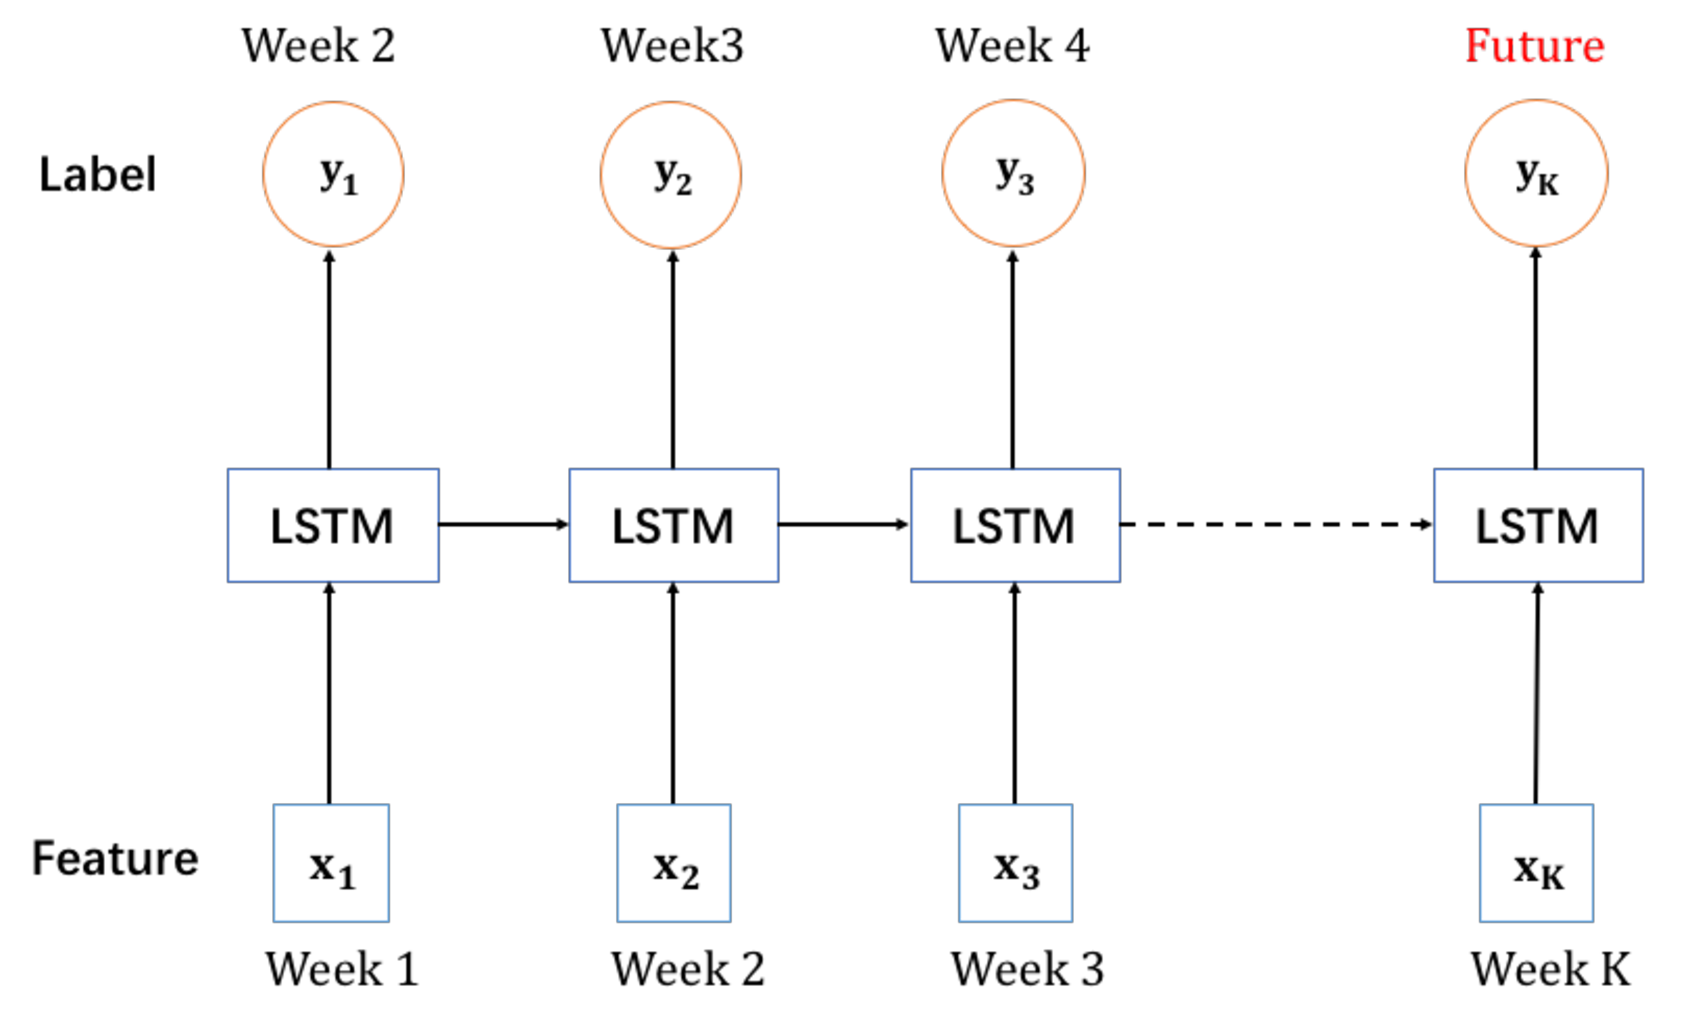
\includegraphics[width=6.4cm, height=3.5cm]{lstm.pdf}
	\caption{LSTM Model for Learning Temporal Patterns From Activity Sequence. We utilize user's Statistics Features in the former week to predict whether he would drop out in the latter week, while we use the features of the last week to predict her dropout in the \emph{future} period.}
	\label{fig:lstm}
\end{figure}
Besides simple statistics, we also adopt LSTM to learn the long-term behavior patterns from the historical activity sequence. LSTM  is an advanced type of recurrent neural network which leverages memory cells and gates to model long-term dependencies within a sequence \cite{Hochreiter1997Long}.  Specifically, Let $\mathbf{S}=(\mathbf{x}_1,\mathbf{x}_2,...,\mathbf{x}_K)$ denote the input sequence, where $\mathbf{x}_k$ is the input vector at position $k$. At each position $k$, there is a set of gate vectors, including input gate $\mathbf{i}_k$, forget gate $\mathbf{f}_k$ and output $\mathbf{o}_k$. It controls for which information should be forgotten, input and output, respectively. Moreover, LSTM adopts a memory cell state $\mathbf{C}_k$ to memorize the internal information at the current time and capture remote dependency. Based on gate vectors and memory cell, the output hidden state $\mathbf{h}_k$ at position $k$ is computed as follows. 
\begin{equation} \mathbf{f}_k = \sigma(\mathbf{W}_f\cdot [\mathbf{x}_k,\mathbf{h}_{k-1}]+\mathbf{b}_f) \end{equation}
\begin{equation} \mathbf{i}_k = \sigma(\mathbf{W}_i\cdot[\mathbf{x}_k,\mathbf{h}_{k-1}]+\mathbf{b}_i) \end{equation}
\begin{equation} \mathbf{C}_k = \mathbf{f}_k \odot \mathbf{C}_{k-1} + \mathbf{i}_t \odot \tanh(\mathbf{W}_c\cdot[\mathbf{x}_k,\mathbf{h}_{k-1}]+\mathbf{b}_c \end{equation}
\begin{equation} \mathbf{o}_k = \sigma(\mathbf{W}_o \cdot [\mathbf{x}_k,\mathbf{h}_{k-1}]+\mathbf{b}_o) \end{equation}
\begin{equation} \mathbf{h}_k = \mathbf{o}_k \odot \tanh(\mathbf{C}_k) \end{equation}
where $\sigma$ is the sigmoid function, $\odot$ is element-wise multiplication, and $\mathbf{W}, \mathbf{b}$ are weight matrices and weight vectors to be learned.\

LSTM is used to learn temporal patterns from user historical activity sequence. The basic idea is to regard this task as a sequential prediction problem and to employ LSTM to predict dropout by weeks.
Specifically, we first partition the \emph{history} period into $K$ weeks $(week_1,week_2,..., week_K)$. For each enrollment $(u,c)$, we utilize Statistics Features in $week_k(1 \le k \le K)$ to predict whether $u$ would drop out in the next week $week_{k+1}$. Whereas we use the features in the last week $week_K$ to predict the real dropout label, which indicates whether $u$ would drop out in the \emph{future} period. Here we use the Statistics Features of historical activity sequence in $k$-th week (described in the previous section), as the input vector $\mathbf{x}_k$ at position $k$. $y_k(1 \le k \le K)$ is defined below.\\
\begin{small}
$$y_k = 
	\begin{cases}
	\text{ 1 if user drops out in  } week_{k+1} \text{ else 0} & \makebox[45pt][r]{$1 \le k \le K-1$} \\
	\text{ 1 if user drops out in }  future \text{ period else 0} & \makebox[30pt][r]{$k=K$}
	\end{cases}
$$
\end{small}
\\
 %The first $K-1$ labels $(y_1, y_2,...,y_{K-1})$ indicate from week sequence $(W_2, W_3,...W_K)$  based on the dropout definition (in Section \ref{ProblemDef}) , whereas $y_{K}$ is the real label which indicates whether $u$ will dropout in $future$ periods. 
 For predicting $y_k(1 \le k \le K)$, the hidden state $\mathbf{h}_k$ at position $k$ is input into a logistics function:
 
\begin{equation}
\hat{y}_k=\frac{1}{1+e^{-\mathbf{w_y}^\mathsf{T} \mathbf{h}_k+b_y}}
 \end{equation}

\noindent where $\mathbf{w_y}$ is the weight vector and $b_y$ is the bias value.
The loss function is defined as:
\begin{equation}
\mathcal{L}(\Theta)= \sum_{k=1}^{K}[y_k\log(\hat{y}_k)+(1-y_k)\log(1-\hat{y}_k)]
\end{equation}
Figure \ref{fig:lstm} presents this model. We use the last prediction probability $\hat{y}_K$ and the last hidden state $\mathbf{h}_K$ as the LSTM Temporal Features.
\subsection{User-related Features}
	\label{sec:UFeat}
	This set of features is extracted from user-course enrollment graph and user profiles. We use these features to capture users' individual information. This type of features is denoted as  $\mathbf{Feat}_u$.\\
	
	\noindent \textbf{User Demographics}\\
    User Demographics (including \emph{gender, age, location, education level}) are extracted from user profiles, and we represent these attributes as a one-hot vector.\\
    
	\noindent \textbf{User Embedding}\\
	Though one-hot representation of a user's demographics can represent the user's necessary information, this method often suffers from sparsity problem in practice, and it could not capture sufficient information about users' preference. Thus we adopt network embedding algorithms to learn features from user-course enrollment graph $G_{uc}$. Similar to those in Section \ref{sec:influence}, we utilize DEEPWALK \cite{Perozzi:2014:DOL:2623330.2623732} to get distributed embedding for each node of $G_{uc}$, and user node embeddings are used as User Embedding features in our framework.\\

	\noindent \textbf{Influence features from friends}\\
	  As we analyzed in section \ref{sec:influence}, user $u$'s behavior in course $c$ is associated with her friends. Thus we design an algorithm to extract influence features from $u$'s friends who have enrolled the same course with her. Following the friends finding method in Section \ref{sec:influence}, for each $u\in \mathbb{U}_c$, we select top $10$ most similar users from her co-learning students set $\mathbb{U}_c-\{u\}$ as her friends. We denote $u$'s friends set as $\mathbb{S}_u=\{u_1, u_2...,u_{N_u}\}$, then the influence features $\mathbf{Feat}_{inf}$ can be calculated based on friends' activity features and similarity scores.
	\begin{equation}
		\mathbf{Feat}_{inf}(u) = \frac{\sum_{i=1}^{N_u} f_s(u, u_i)\mathbf{Feat}_{stat}(u_i)}{\sum_{i=1}^{N_u} f_s(u, u_i)}
	\end{equation}
	where $\mathbf{Feat}_{inf}(u)$ denotes the influence feature of $u$, $\mathbf{Feat}_{stat}(u_i)$ is the Statistics Features (Section \ref{sec:activityFeat}) of $u_i$, and $f_s$ is the similarity function, which is cosine function between the two node vectors.
	
\subsection{Course-related Features}
	\label{sec:CFeat}
	Similar to the User-related features, we also design a set of features to represent course specific information. This set of features is defined as $\mathbf{Feat}_c$.\\
	
	\noindent \textbf{Course Category}\\
	These features are acquired based on the courses categorization scheme provided by XuetangX, which categorizes the courses into twelve types (described in Section \ref{sec:XuetangX}). We also use a $12$-dim one-hot vector to represent each course's category in our framework.\\
	
	\noindent \textbf{Course Embedding}\\
	Similar to the User Embedding in Section \ref{sec:UFeat}, the embeddings of courses obtained from user-course enrollment graph are used as preference features from the perspective of course. \\
%from the dimension of course
 
     %\section{Co-training Framework}
	\label{sec:Co-Train}
	\begin{figure}
	\centering 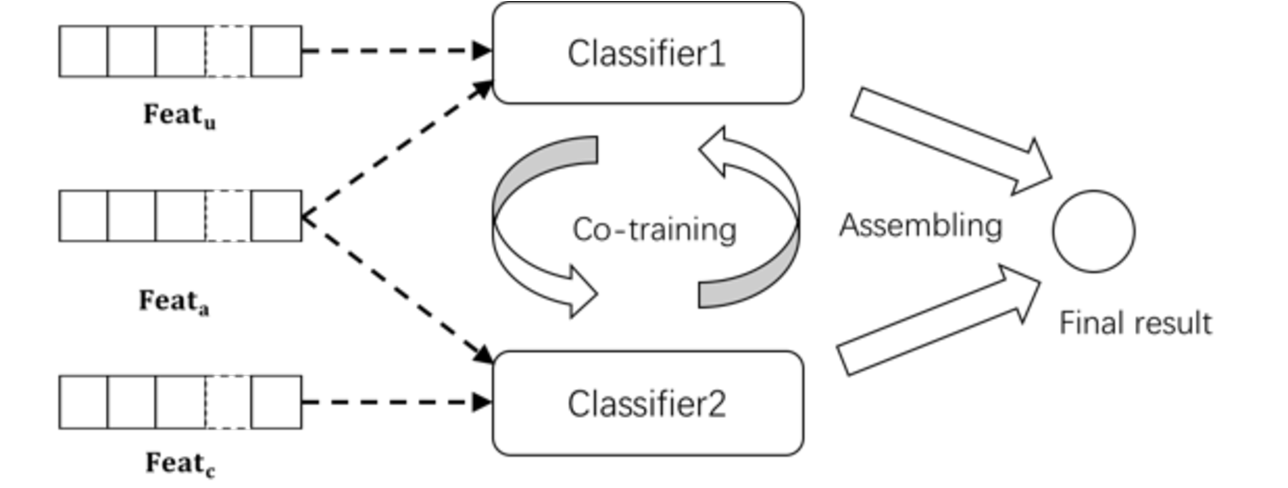
\includegraphics[width=9cm]{architecture.pdf}
	\caption{The Illustration of Dropout Prediction Framework.}
	\label{fig:arch}
	\end{figure}
	In order to combine features extracted from different sources, we design a multiview based Co-training framework. There are two classifiers in this framework. One is used to learn user individual preference, while the other one is to learn course-related preference.  Moreover, the Co-training framework can leverage unlabeled data to facilitate the prediction performance on the sparse personalized data. Specifically, Co-training framework consists of three steps.
	\begin{itemize}
		\item {\textbf{Constructing multiple classifiers.}} The first step is to construct multiple classifiers with good diversity based on the three types of features: $\mathbf{Feat}_a$, $\mathbf{Feat}_u$ and $\mathbf{Feat}_c$.
		
		\item{\textbf{Co-Training.}} In the Co-Training procedure, each classifier can learn from each other. More accurately, those examples with high confidences are selected for the classifier and being labeled based on the predict probability score,  and then they are used to ``teach" the other classifier.
		\item{\textbf{Assembling the results.}} In the end, the probability scores obtained by individual classifiers are assembled to the final prediction score.
	\end{itemize}
	Algorithm \ref{alg:Co-Training} gives the details of the Co-training algorithm, and the whole architecture of our dropout prediction framework is illustrated in Figure \ref{fig:arch}.
	\begin{algorithm}[!h]
		\caption{Co-Training Algorithm.}  
		\label{alg:Co-Training}  
		\KwIn{the training set $L$, and the test example set $U$;}
		\KwOut{classifier $h(u,c)$ for dropout prediction;}
		\textbf{Step 1: Construct Multiple classifiers}\\
		Generate two classifiers $h_1$ and $h_2$ based on multiviews;\\
		Initialize the training sets of $h_1$ and $h_2$: $L_1=L $, $L_2 = L$; \\  
		Create a pool $U'$ by randomly picking $\mathcal{U}$ examples from $U$;\\
		\textbf{Step 2: Co-Training}\\
		\Repeat{$\mathcal{T}$ rounds}{
			\For {j=1 to 2}{
				Training $h_j$ on the corresponding training set $L_1$ and labeling the examples in $U'$;\\
				Constructing teaching set $T_j$ by selecting $p$ positive and $n$ negative examples from $U'$;\\
				$U' = U'-T_j$;
			}
		    Randomly choose $2p+2n$ examples from $U$ to replenish $U'$\\
			Teach peer classifiers: $L_1=L_1 \cup T_2$; $L_2=L_2 \cup T_1$;\\
			%Update the two classifiers: $h_1\leftarrow L_1$; $h_2\leftarrow L_2$;
		}
		\textbf{Step 3: Assembling the results} $h(u,c)=Assemble(h_1(u,c), h_2(u,c))$
	\end{algorithm}

	
	\subsection{Constructing multiple classifiers}
	\label{sec:construct}
	Generating multiple classifiers with good diversity is the key point in the Co-training framework. Here we employ a multiview based method to construct different classifiers. Multiview mechanism has been widely used in many different machine learning topics. Here we adopt this method to construct different classifiers. In this method, all features (described in Section \ref{sec:allFeat})  are divided into two sets: $\{\mathbf{Feat}_a, \mathbf{Feat}_u\}$ and $\{\mathbf{Feat}_a, \mathbf{Feat}_c\}$. Then the two sets of features are input to two different classifiers, respectively. We denote the two classifiers as $h_1$ and $h_2$, and they can be formalized as follows.
	\begin{equation}
	h_1(u,c) = g([\mathbf{Feat}_{a}, \mathbf{Feat}_{u}])\end{equation}
	\begin{equation}h_2(u,c)=g([\mathbf{Feat}_{a}, \mathbf{Feat}_{c}])
	\end{equation}
	Where $g(\cdot)$ is the classify function. $h_1$ is used to capture individual preference from the perspective of user, while $h_2$ is learning course-related preference information. Based on previous work\cite{Zhou:2005:SRC:1642293.1642439}, each learner of the Co-training framework should be sufficient for each learner in the Co-training framework to learn. In order to meet the requirement, Activity Features $\mathbf{Feat}_a$ are input to both classifiers as the extra feature set. 
	
	\subsection{Semi-supervised Co-training}
	\label{sec:co-training}
		After constructing multiple classifiers, the task amounts to co-training the different classifiers. For each classifier $j$, we need to construct a ``teaching set" $T_j$ from the unlabeled samples and use it to teach the other classifier. Before that, we must label the unlabeled examples based on the classification confidences produced by each classifier. Moreover, In order to make this procedure more efficient, a smaller pool set $U'$ is drawn randomly from the whole unlabeled set $U$ before co-training. This was proved to be helpful for improving the final performance in the previous work\cite{Blum:1998:CLU:279943.279962}.\\
	
	\noindent \textbf{Labeling the unlabeled examples}
    
	Labeling is the final step for most of the classifier systems, in which the unlabeled samples are labeled based on their classification scores. For binary classification, a general labeling strategy is to compare classification score with a decision threshold $\gamma$. If the score of an example is higher than $\gamma$, then the example is set to positive, otherwise, it is set to negative. $\gamma$ is usually set to $0.5$ when the classification score is from $0$ to $1$.  However, this strategy does not work on the imbalanced datasets of dropout prediction task. To alleviate the imbalanced classification problem, we propose a ranking based labeling strategy with three steps:
	\begin{itemize}
		\item Calculate the ratio $r$ of positive examples to all examples in training set: $r=\frac{|P_L|}{|N_L|+|P_L|}$, where $P_L$ is the set of positive examples and $N_L$ is the set of negative examples.
		\item Rank all the examples in $U'$ using their classification score.
		\item Label top $r * |U'|$ examples in $U'$ as positive, and others as negative.
	\end{itemize}
    Next, the classification confidence of example $x_{uc}$ predicted by classifier $j$ is:
    \begin{equation}
    C_j(x_{uc})=l_{x_{uc}}*s_{x_{uc}} + (1-l_{x_{uc}})*(1-s_{x_{uc}})
    \end{equation}
    where $s_{x_{uc}}$ is the classification score of $x_{uc}$, and $l_{x_{uc}} \in \{0,1\}$ is its corresponding label. $l_{x_{uc}} = 1$ means $x_{uc}$ is positive, while $l_{x_{uc}} = 0$ indicates that the example is negative. As shown above, if $x_{uc}$ is labeled to positive, the corresponding confidence is  its classification score $s_{x_{uc}}$, and if $x_{uc}$ is negative, its confidence is $1- s_{x_{uc}}$.\\
    
    
    \noindent \textbf{Constructing Teaching Set and Co-training}
    
    For constructing the ``teaching set'' $T_j$ for each classifier $j$, we adopt Roulette algorithm \cite{Back:1996:EAT:229867} to sample examples randomly from $U'$ based on their confidences. The sample probability of each example is calculated by:
     \begin{equation}
     Pr(x_{uc}, j)=\frac{C_j(x_{uc})}{\sum_{x_i\in U'}C_j(x_i)}
     \end{equation}
     We sample $p$ positive examples and $n$ negative examples to construct $T_j$ for each classifier $j$.
    After selecting examples from $U'$, we need to choose $2p+2n$ examples from test set $U$ to replenish $U'$. Finally the examples in one teaching set $T_j$ are merged into the training set of the other classifier. In this way, the unlabeled data are incorporated into the learning process. This procedure of constructing the teaching sets and Co-training will be repeated for $\mathcal{T}$  iterations in this algorithm.
    \subsection{Assembling the Results}
    \label{sec:assemble}
    The results of two classifiers are assembled together in the final step. A general method is to compute the mean value for all the classification scores, i.e.,
    \begin{equation}
    h(u,c) =\frac{1}{l}\sum_{j=1...l}h_j(u, c)
    \end{equation}
    
    where $l$ is the number of classifiers being assembled. In our case, the ensemble scheme for two classifiers is $h(u,c) = \frac{1}{2}[h_1(u,c)+h_2(u,c)]$. However, this method does not consider the classification confidence of different classifiers. To address this problem, we assemble the results by taking weighted average of all results. Here the weights are computed by the classification confidences, i.e.,
    \begin{equation}
    h(u,c)=\sum_{j=1...l}\frac{C_j(x_{uc})}{\sum_{k=1...l}C_k(x_{uc})}h_j(u,c)
    \end{equation}
    Another option for computing weights is based on the average AUC score of k-fold cross validation: $h(u,c)=\sum_{j=1...l}\frac{w_j}{\sum_{k=1...l}w_k}h_j(u,c)$. Where $w_j$ is the average AUC score of the $h_j$'s k-fold cross validation on training set. However, running k-fold cross validation means that the model must be trained $k$ times on training set, which is less efficient in practice. 
    Note that these ensemble methods can either be applied right after the training of individual models without the Co-training. By this way, the framework only makes use of the labeled data, while the Co-training framework can consider not only labeled data but also unlabeled data.
     %\section{Experiments}
We conduct various experiments to evaluate the effectiveness of the extracted features and Co-training framework on both \textit{KDDCUP Dataset} and \textit{XuetangX Large-Scale Dataset}.

\subsection{Experimental Setup.} 
	\noindent\textbf{Classifier.}
	We use XGBoost as the classifier in our experiments, XGBoost is short for eXtreme Gradient Boosting\cite{Chen:2016:XST:2939672.2939785} which is an optimized distributed gradient boosting system with high efficiency, flexibility, and portability. It was implemented under the Gradient Boosting framework\cite{Friedman2001Greedy}. \\
    %Comparing with the original Gradient Boosting algorithm, XGBoost utilize a more regularized model formalization to control over-fitting, which gives a better performance. \\
    
	\noindent \textbf{Comparison Methods.}
	We conduct the comparison experiments for testing Co-training performance with the following methods:
	\begin{itemize}
		\item{\textbf{Logistic Regression Classifiers (LRC)}}: The logistic regression model is used to predict user's dropout.
		\item{\textbf{SVM}}: A linear kernel SVM is trained for predicting the dropout probability of each user.
		\item{\textbf{Random Forest (RF)}}: All features are input to a Random Forest model to predict dropout probability.
		\item{\textbf{XGBoost (XGB)}}: A single XGBoost model is used for this task.
		\item{\textbf{Ensemble XGBoost ($\mathbf{XGB_{en}}$)}}:  Assembling $h_1$ and $h_2$ directly (Section \ref{sec:construct}) with XGBoost as the classifiers. The ensemble strategy is Average Weighted.
		\item{\textbf{Co-training XGBoost ($\mathbf{XGB_{co}}$)}}: The Multi-view Co-training algorithm (in Section \ref{sec:co-training}) by adopting XGBoost as classifier.
\end{itemize}	
	For single models(\textbf{LRC, SVM,  RF, XGB}) above, we use all the features described in Section \ref{sec:allFeat} (including $\mathbf{Feat}_{a}, \mathbf{Feat}_{c}, \mathbf{Feat}_{u}$) as input. 
	When training the models,  we tune the parameters using the average AUC on 5-fold cross validation(CV) with grid search algorithm, and use the best group of parameters in all experiments.\\
	
	\noindent \textbf{Evaluation Measures.} We evaluate the classification performance by using the Area Under the ROC Curve(AUC) and F1 Score(F1).
	
	\subsection{Co-training performance}
	
	\begin{table}
		\centering
		\caption{Overall Results on KDDCUP Dataset and Instructor-paced courses of XuetangX Large-Scale Dataset. }
		\begin{tabular}{c|cc|cc}
			\hline \hline
			              &\multicolumn{2}{c|}{KDDCUP} &\multicolumn{2}{c}{XuetangX}\\
			  Methods & AUC & F1 & AUC & F1  \\

			 \hline
			  LRC                      & 86.78 & 90.8:6   &  80.77 &91.42 \\
			 \hline
		     SVM                   &  89.56  & 91.75	   &   81.13  &91.37 \\
			\hline
			RF                       & 88.82  & 91.73  &82.72  &92.01 \\
			\hline
			 XGB 					&90.51 &92.78   & 83.53& 92.08\\
			\hline
			$\rm XGB_{en}$  &90.53  &92.80  & 83.56  &92.10\\
			\hline
		    $\rm XGB_{co}$ &\textbf{90.94} & \textbf{93.19} & \textbf{84.27}& \textbf{92.23} \\ 
			\hline	\hline
		\end{tabular}

		\label{tab:allRes}
	\end{table}
	

	Table \ref{tab:allRes} presents the results on \textit{KDDCUP Dataset} and Instructor-paced courses of \textit{XuetangX Large-Scale Dataset} for all comparison methods. Overall, $\rm XGB_{co}$ gets the best performance on both two datasets, and its AUC score on KDDCUP dataset achieves 90.94\%  which is comparable to the winner team of KDDCUP 2015\footnote{https://biendata.com/competition/kddcup2015/rank/}. Compared to LRC and SVM, $\rm XGB_{co}$ achieves 1.38-4.16\% and 3.14-3.50\% AUC score improvements on KDDCUP dataset and XuetangX dataset, respectively.
  Random Forest and single XGBoost model also underperform. Moreover, by comparing the performance of XGB and $\rm XGB_{en}$, we find that assembling different views of XGBoost models only contributes limited improvements on this task. Again, it indicates that Co-training procedure, which makes use of unlabeled data, is helpful for enhancing the ensemble results.
	
	
	\begin{table}
		\caption{Feature Ablation Results on KDDCUP Dataset and Instructor-paced courses of XuetangX Large-Scale Dataset.}
		\centering
		\begin{tabular}{llcccc}
		\hline \hline
			&               & \multicolumn{2}{c}{KDDCUP} & \multicolumn{2}{c}{XuetangX} \\
			\multicolumn{2}{l}{Features}                &AUC    & F1   & AUC    & F1   \\ \hline 
			\multicolumn{2}{l}{All}                     & 90.51 & 92.78 & 83.53 & 92.08     \\ \hline
			\multicolumn{2}{l}{- Activity}          &  87.76 & 91.21     &80.13	  &91.35   \\ 
			& - Statistics                            & 88.78 & 91.43    &81.73   & 91.70  \\
			& - LSTM                              & 90.22  & 92.61     & 81.70  & 91.69    \\ \hline
			\multicolumn{2}{l}{- User}           &90.08  &92.56    & 81.97  & 91.73      \\
			& - Demographics                       & 90.49  & 92.77     & 83.50 & 92.06      \\ 
			& - Embedding                            & 90.26  & 92.66     & 82.82  & 91.89  \\ 
			& - Influence                              &   90.23   & 92.65     & 82.84    &91.90  \\ \hline
			\multicolumn{2}{l}{- Course}      & 90.02    & 92.45    & 81.80    & 91.71   \\
			& - Category                              & 90.45       &92.75     &83.47   &92.05   \\ 
			& - Embedding                          &   90.21        &92.64      &82.83  &91.90           \\ \hline \hline
 \end{tabular}

	  \label{tab:featImp}	
	\end{table}
	\subsection{Feature Importance}
	In order to analyze the importances of different types of features, we conduct the feature ablation experiments on \textit{KDDCUP Dataset} and Instructor-paced courses of \textit{XuetangX Large-Scale Dataset}. Specifically, we first input all the features to the XGBoost classifier, then remove every type of features one by one to watch the variety of performance.
	The ablation results are shown in Table \ref{tab:featImp}. We observe that all types of features are useful for these two datasets. Compared to User-related Features and Course-related Features, Activity Features are more important for this problem. For Activity Features, Statistical Features help improvement more than LSTM Features on \textit{KDDCUP Dataset}, though LSTM shows a bit better performance on \textit{XuetangX Large-Scale Dataset} than statistics. This is because that \textit{XuetangX Large-Scale Dataset} has much more training examples which can help LSTM get a better generalization. Moreover, Embedding Features for User and Course achieve a better performance than traditional One-hot Features (including User Demographics and Course Category), and the Influence Features from Friends also contribute to the improvement on these two datasets.
	\subsection{Discussion for Self-paced Courses}
	
		\begin{table}
		\centering
		\caption{Results on Self-paced Courses }
		\begin{tabular}{ccccccc}
			\hline
			\hline
			Methods & LRC & SVM &RF & XGB &$\rm XGB_{en}$& $\rm XGB_{co}$ \\
			\hline
			AUC    & 69.76 & 71.23 & 72.34 &73.67 & 74.10 & 74.27 \\
			\hline
			\hline		
		\end{tabular}

		\label{tab:selfRes}
	\end{table}
	Besides experiments on Instructor-paced courses, we also conduct the same experiments on Self-paced courses of \textit{XuetangX Large-Scale Dataset}. As shown in table \ref{tab:selfRes}, all the prediction results on Self-paced courses are rather lower than the results on Instructor-paced courses (table \ref{tab:allRes}). This is because Self-paced courses give more freedom to students, and do not require students to learn within a specified time. Therefore, there are more uncertainty for dropout prediction on Self-paced courses.


    %This is because of the big difference between this two kinds of courses: Instructor-paced courses follow a schedule that the instructor sets, assignments and exams of which have specific due dates. 
	\begin{figure}
		\centering
		\includegraphics[width=4.5cm,height=3.5cm]{snapshot.pdf}
		
		\caption{A Snapshot of the Online System. If a user is identified as risk of dropout by our prediction framework, LittleMu will remind the user that there are some new materials updated on the course.} 
		\label{fig:snapshot}
	\end{figure}
	\subsection{Online System}
	We deployed our framework on the \textit{LittleMu} system, an intelligent teaching assistant system on XuetangX, for facilitating user retention.
	Specifically, for each course, we first provide online dropout prediction for all enrolled users. Then if a user's dropout probability is greater than a threshold, LittleMu would remind her to learn on the courses by sending him a message: \emph{``There are some new materials updated on the course, do you want to take a look?''}. Figure \ref{fig:snapshot} shows a snapshot of the system. This strategy is
based on our investigation for students' dropout reasons on XuetangX,  of which results indicate that over
20\% students drop out from XuetangX because no one remind them to learn on their enrolled courses.
		
     
     %%deep model version:
     \section{Methodology}
\hide{
\begin{table}[]
    \caption{Notation Description}
    \centering
    \begin{tabular}{c|c}
    \hline
       $\mathbf{X}_{\alpha}$  & activity feature \\ \hline
       $\mathbf{X}_{\alpha}^{(i)}$ & $i^{th}$ feature group of activity feature \\ \hline
       $\mathbf{X}_{\beta}$  & user-specific feature \\ \hline
       $\mathbf{X}_{\gamma}$   & course-specific feature \\ \hline
       $\textbf{E}^{(i)}_\alpha$ & embedding of $\mathbf{X}_{\alpha}^{(i)}$ \\ \hline
       $\mathbf{E}_\beta$ & embedding of   $\mathbf{X}_{\beta}$ \\ \hline
        $\mathbf{E}_\gamma$ & embedding of   $\mathbf{X}_{\gamma}$ \\ \hline
         $\textbf{V}_\alpha$ &  activity feature maps \\ \hline
       $\mathbf{V}_\beta$ & user-specific feature map \\ \hline
        $\mathbf{V}_\gamma$ & course-specific feature map\\ \hline
    \end{tabular}
    \label{tab:my_label}
\end{table}
}
We now turn to discuss potential solutions to predict when and whether a user will drop out a specific course, 
by leveraging the patterns discovered in the above analysis. In summary, we propose a Context-aware Feature Interaction Network (\modelname{}) to deal with the dropout prediction problem. Different from previous work on this task, the proposed model incorporates context information, including user and course information, into a unified framework. Let us begin with a formulation of the problem we are going to address.

\subsection{Formulation}
	\label{ProblemDef}
	

\begin{figure}
	\centering
	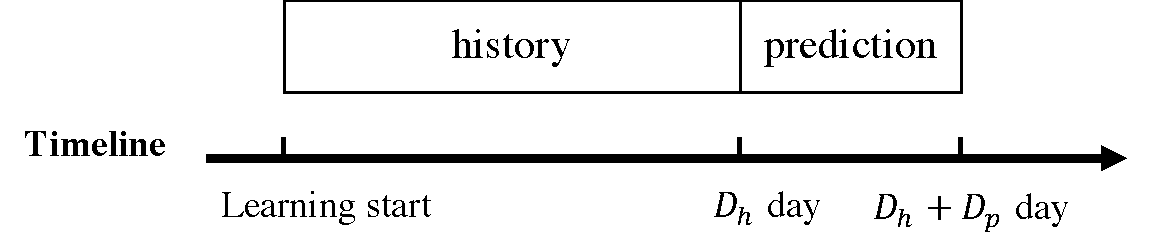
\includegraphics[width=0.8\linewidth]{course-span.pdf}
	
	\caption{Dropout Prediction Problem. The first $D_h$ days are \emph{history period}, and the next $D_p$ days are \emph{prediction period}.}
	\label{fig:dataCons}
\end{figure}
\hide{
	\item{Activity Count/Ratio:} For each enrollment $(u,c)$, we calculate the number and ratio for each type of activities in table \ref{ResourceAction}. 
\item{Activity Temporal Statistics:} The whole duration time of a course is divided by weeks, and the activity counts and statistics(including \emph{max, min, stdev, median}) in different weeks are used as features.
\item{Activity Count in Hours Per Day:} We calculate user activity count for each hour in a day (24 hours).
\item{Activity Count in Day Per Week:} We compute user activity count for each day in a week (5 weekdays + 2 weekends).
\item{Activity N-gram Count/Ratio:} The N-grams of activity sequence is used to capture the correlations between neighbor activities. We employ N-gram activity count and ratio as the N-gram features.
\item{Engagement Style:} Following the taxonomy of engagement introduced by Anderson et al. \cite{Anderson:2014:EMO:2566486.2568042ß}, we use the $\emph{assignment fraction} = \frac{ \emph{watching video \#}}{ \emph{complete assignment \#}}$ to represent user's engagement pattern.
\item{Learning Time Span:} A user's learning time span is the duration between a user's first visit time and her last visit time on a course.  

\item{Effective Learning Time:} The \emph{effective learning time} introduced by Qiu et al. \cite{Qiu:2016:MPL:2835776.2835842} is an approximated method to compute user's actual study time on a certain course. This is calculated based on the time interval between user's \emph{watching video} and \emph{stop video}, and we employ this feature in our paper.

\item{Visiting Time Interval:} A user's interval time for visiting one course reflects user's interests in this course. The statistics(\emph{max, min, stdev, median}) of visiting time intervals are used as features.\\
}
\hide{
\begin{table*}[]
	\caption{Activity Features}
	\centering
	\begin{tabular}{p{3.7cm}|p{13.4cm}}
		\hline
		Activity Count/Ratio  &  Total number and ratio of each type of learning activities\\ \hline
		Activity Temporal Statistics&  The whole duration time of a course is divided by weeks, and the activity counts and statistics(including \emph{max, min, stdev, median}) in different weeks are used as features.\\ \hline
		Activity Count Per Hour  &  The number of users' learning activities for each hour in a day (24 hours).\\ \hline
		Activity Count Per Day & The number of users' learning activities for each day in a week (5 weekdays + 2 weekends). \\ \hline
		Activity N-gram Count/Ratio & The N-grams of activity sequence is used to capture the correlations between neighbor activities. We employ N-gram activity count and ratio as the N-gram features. \\ 
	 \hline
		Engagement Style & Following the taxonomy of engagement introduced by Anderson et al. \cite{Anderson:2014:EMO:2566486.2568042ß}, we use the $\emph{assignment fraction} = \frac{ \emph{watching video \#}}{ \emph{complete assignment \#}}$ to represent user's engagement pattern.  \\ \hline
		Learning Time Span & A user's learning time span is the duration between a user's first visit time and her last visit time on a course.  \\ \hline
		Effective Learning Time & The \emph{effective learning time} introduced by Qiu et al. \cite{Qiu:2016:MPL:2835776.2835842} is an approximated method to compute user's actual study time on a certain course. This is calculated based on the time interval between user's \emph{watching video} and \emph{stop video}, and we employ this feature in our paper.\\ \hline
		Visiting Time Interval & A user's interval time for visiting one course reflects user's interests in this course. The statistics(\emph{max, min, stdev, median}) of visiting time intervals are used as features.
		\\ \hline
	\end{tabular}
	\label{tab:acvtityFeat}
\end{table*}
}
%Our main task is to predict whether a user would dropout from an enrolled course in a pre-specified time window. 
In order to formulate this problem more precisely, we first introduce the following definitions. 

\emph{Definition 2.} \textbf{Enrollment Relation}: Let $\mathbb{C}$ denote the set of courses, $\mathbb{U}$ denote the set of users, and the pair $(u,c)$ denote user $u\in \mathbb{U}$ enrolls the course $c\in \mathbb{C}$.
The set of enrolled courses by $u$ is denoted as  $\mathbb{C}_u\subset \mathbb{C}$ and 
the set of users who have enrolled course $c$ is denoted as $\mathbb{U}_c\subset \mathbb{U}$.
We use $\mathbb{E}$ to denote the set of all enrollments, i.e., $\{(u,c)\}$

\emph{Definition 3.} \textbf{Learning Activity}: 
In MOOCs, user $u$'s learning activities in a course $c$ can be formulated into an $m_x$-dimensional vector $\mathbf{X}(u,c)$, where each element $x_i(u,c) \in \mathbf{X}(u,c)$ is a continuous feature value associated to $u$'s learning activity in a course $c$. Those features are extracted from user historical logs, mainly includes the statistics of users' activities.

\emph{Definition 4.} \textbf{Context Information}: Context information in MOOCs comprises user and course information. User information is represented by user demographics (i.e. gender, age, location, education level) and user cluster. While course information is the course category. The categorical information (e.g. gender, location) is represented by a one-hot vector, while continues information (i.e. age) is represented as the value itself. By concatenating all information representations, the context information of a $(u,c)$ pair is represented by a vector $\mathbf{Z}(u,c)$.   


%Activity pattern vector mainly includes users' learning behavioral features, which are extracted from user historical activity logs. The details are exhibited in Table \ref{tab:acvtityFeat}. User-related pattern vector consists of user demographics (i.e. gender, age, location, education level and user id) and user cluster (Cf. Section \ref{sec:temporal}). Course-related pattern vector,  including course id and course category, is used to represent course specific information in MOOCs. \\
%Specifically the pattern vector includes three types of patterns: activity pattern vector $\mathbf{X}_a \in \mathbb{R}^{m_a}$, user-specific pattern vector $\mathbf{X}_u \in \mathbb{R}^{m_u}$ and course-specific pattern vector $\mathbf{X}_c \in \mathbb{R}^{m_c}$.  

% into a paired tuple  $x = (a, t)$, where $a$ represents user's action(such as ``watching video'') and $t$ is the corresponding logged time stamp. In this paper, we focus on four types of learning activities: \emph{video, forum, assignment, web page}, which are described in table \ref{ResourceAction}. \\

%Each course has a set of available resources for users, such as video and forum. Here we use $R$ to represent the resource set of course on MOOCs. For each resource $r \in R$, there are a set of specific actions for it. We use $A$ to denote the action set. In this paper, we focus on four types of resources on MOOCs: \emph{video, forum, assignment, web page}, which are shown in table \ref{ResourceAction}, together with the corresponding actions. 

%Then a learning activity record of $u\in \mathbb{U}$ in one enrolled course $c\in \mathbb{U}_c$ at time $t$ can be represented as $X=(u,c,r,a,t)$, where $r\in R$ is the resource $u$ has accessed, $a\in A$ is the corresponding action on $r$. For each $(u,c) \in \mathbb{E}$, we use $\mathcal{X}_{uc}$ to represent user $u$'s historical learning activity set on $c$.\\

With these definitions, our problem of dropout prediction can be defined as: Given user $u$'s learning activity $\mathbf{X}(u,c)$ on course $c$ in \textit{history period} (as shown in Figure \ref{fig:dataCons}, it is the first $D_h$ days after the learning starting time), as well as her/his context information $\mathbf{Z}(u,c)$, our goal is to predict whether $u$ will drop out from $c$ in the \textit{prediction period} (as shown in Figure \ref{fig:dataCons}, it is the following $D_p$ days after \textit{history period}). More precisely, let $y_{(u,c)} \in \{0,1\}$ denote the ground truth of whether $u$ has dropped out, $y_{(u,c)}$ is positive if and only if $u$ has not taken activities on $c$ in the \textit{prediction period}. Then our task is to learn a function:
%Given user $u$'s activity sequence $X_{(u,c)}= [x_1, x_2,...,x_N]$ on course $c$ in \textit{history period}(as shown in Figure \ref{fig:dataCons}, it is the first $D_h$ days after the learning starting time), our goal is to predict whether $u$ will drop out from $c$ in the \textit{prediction period}(as shown in Figure \ref{fig:dataCons}, it is the following $D_p$ days after \textit{history period}). More precisely, let $y_{(u,c)} \in \{0,1\}$ denote the ground truth of whether $u$ has dropped out, $y_{(u,c)}$ is positive if and only if $u$ has not taken activities on $c$ in the \textit{prediction period}. Then our task is to learn a function:

$$f: (\mathbf{X}(u,c), \mathbf{Z}(u,c))\to y_{(u,c)}$$ 

\hide{Let $\mathbb{C}$ denote the set of courses, $\mathbb{U}$ denote the set of users, and the pair $(u,c)$ denote user $u\in \mathbb{U}$ enrolls the course $c\in \mathbb{C}$.
The set of enrolled courses by $u$ is denoted as  $\mathbb{C}_u\subset \mathbb{C}$ and 
the set of users who have enrolled course $c$ is denoted as $\mathbb{U}_c\subset \mathbb{U}$.
We use $\mathbb{E}$ to denote the set of all enrollments, i.e., $\{(u,c)\}$.
Given this, our problem of dropout prediction can be defined as:}

\hide{
	   \emph{Definition 2.} \textbf{$t$-Dropout Prediction}: Given all users $\mathbb{U}$'s learning activity $\textbf{X}^t$ in all courses $\mathbb{C}$ before time $t$, our goal is to learn a function $f$ in order to infer
	   $$f: (\mathbb{U},\mathbb{C},\textbf{X}^t)\to \{y^t_{(u,c)}\}$$
	   \noindent where $y_{(u,c)} \in \{0,1\}$ indicates whether user $u$ would drop out ($y=1$) course $c$ 
	   after time $t$ or not. 
}
\hide{
	   sequence $X_{(u,c)}= [x_1, x_2,...,x_N]$ on course $c$ in \textit{history period}(as shown in Figure \ref{fig:dataCons}, it is the first $D_h$ days after the learning starting time), our goal is to predict whether $u$ will drop out from $c$ in the \textit{prediction period}(as shown in Figure \ref{fig:dataCons}, it is the following $D_p$ days after \textit{history period}). More precisely, let $y_{(u,c)} \in \{0,1\}$ denote the ground truth of whether $u$ has dropped out, $y_{(u,c)}$ is positive if and only if $u$ has not taken activities on $c$ in the \textit{prediction period}. Then our task is to learn a function:
	 $$f: (u,c,X_{(u,c)})\to y_{(u,c)}$$
}    

	
\hide{
Based on the analyses in previous section, users' dropout in a course has high correlation with their context(similar courses and friends). How to construct a personalized prediction system for diverse users in MOOCs is a quite difficult problem. In this section, we introduce our methodology of personalized dropout prediction. We consider three types of features, i.e., activity features, user-related features and course-related features, when predicting users' dropout.
}
\hide{
  \begin{table}
	\hspace{-0.01in}
	\centering
	\caption{Average activity feature values on two sample courses --- Conversational English and Data Structure. CAR --- average correct answer ratio. }
	\small
	\label{tab:sample}
	\setlength{\tabcolsep}{1mm}\begin{tabular}{@{}c@{}|l@{}|c|c}
		\hline
		\hline
		Category &  Type   & Conversational English & Data Structure \\
		\hline
		\multirow{3}{*}{video}&  \#watch &74.80 & 32.48\\	
		\cline{2-4}
		& \#stop     &69.53 & 26.14\\
		\cline{2-4}
		& \#jump   &51.18 & 14.38\\
		\hline
		\multirow{2}{*}{forum}&  \#question & 0.049 & 0.038 \\
		\cline{2-4}
		& \#answer &1.10&0.12 \\
		\hline
		\multirow{2}{*}{assignment} & CAR &0.45 & 0.41 \\
		\cline{2-4}
		& \#revise  &0.09& 0.02 \\
		\hline
		\multirow{2}{*}{session}    & seconds &1,715 &714 \\
		\cline{2-4}                
		&  count     &3.61 &8.13 \\  
		\hline
		\multicolumn{2}{c|}{dropout rate} &0.74 &0.73 \\
		\hline	
		\hline
	\end{tabular}
	\normalsize
\end{table}
}

Please note that we define the prediction of dropouts for all users/courses together, as we need to consider the user and course information. 
%In next section, we will explain the details of our solution --- Context-aware Feature Interaction Network --- for this task.


%Another challenge we have to face is how to incorporate the course correlation and friend influence into the prediction. To solve these challenges, we proposed an Attention-based Feature Interaction Network (AFIN) to predict dropout by incorporating users' context information.
\subsection{Context-aware Feature Interaction Network}
 \begin{figure}
	\hspace{-0.1in}
	\centering
	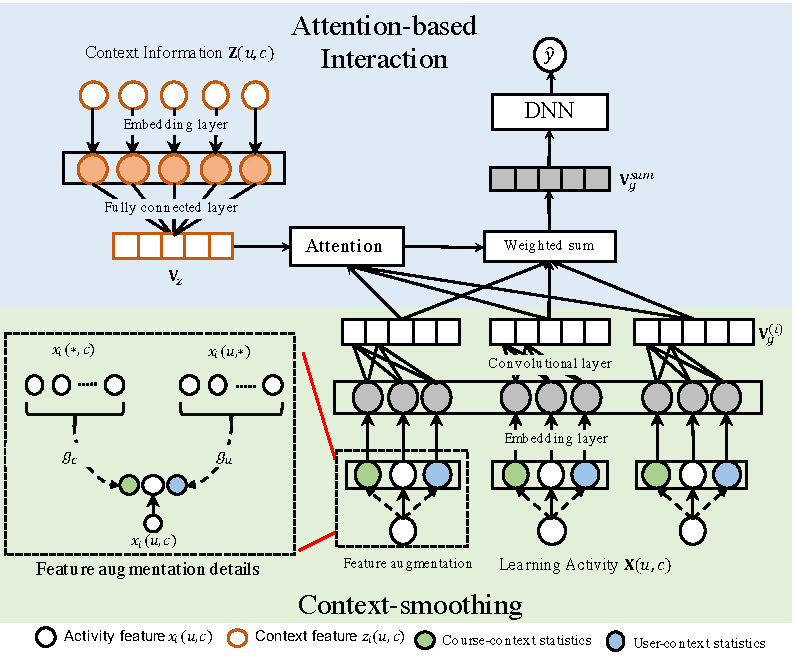
\includegraphics[width=\linewidth]{model_arch_new.pdf}	
	\caption{The architecture of \modelname{}.}
	\label{fig:modelArch}
\end{figure}
\vpara{Motivation.} From prior analyses, we find users' activity patterns in MOOCs have a strong correlation with their context (e.g. course correlation and friends influence). More specifically, the value of learning activity vector $\textbf{X}(u,c)$ is highly sensitive to the context information $\textbf{Z}(u,c)$. 
\hide{
For example, the average activity features of table \ref{tab:sample} presents the average activity feature values of two sample courses of XuetangX (i.e. Conversational English and Data Structure). We observe that these features are totally different between two courses though they have approximate user dropout rates.}
To tackle this issue, we employ convolutional neural networks (CNN) to learn a context-aware representation for each activity feature $x_i(u, c)$ by leveraging its context statistics. This strategy is referred to as context-smoothing in this paper. What's more, we also propose an attention mechanism to learn the importances of different activities by incorporating $\textbf{Z}(u,c)$ into dropout prediction. Figure~\ref{fig:modelArch} shows the architecture of the proposed method.  In the rest of this section, we will explain the context-smoothing and attention mechanism in details.
%However,  very few works have attempted to incorporate the context information into the dropout prediction framework.
% This is the main motivation for our approach. 
 
 %More specifically, we found the value of the learning activity vector $\textbf{X}(u,c)$ is highly sensitive to the context information $\textbf{Z}(u,c)$. Table \ref{tab:sample} presents an example of the average activity feature values on two courses (i.e. Conversational English and Data Structure). We can observe that these features are totally different between two courses though they have a approximate user dropout rate. A general solution for this challenge is to augment the learning activity vector with its statistics of user-level and course-level and feed the augmented learning activity vector into the classifier directly. However, it always suffers from the curse of dimensionality and can not get a better performance. To tackle this issue, we employ convolutional neural networks (CNN) to learn a context-aware representation for each activity feature of $\textbf{X}$ by leveraging its context statistics. This strategy is referred to context-smoothing in this paper. What's more, we also propose an attention mechanism to learn the importances of different activities by incorporating the context information into dropout prediction. Figure~\ref{fig:modelArch} shows the architecture of the proposed method.

%The main technical contributions of Attention-based Feature Interaction Network (AFIN) lies in the proposal of context-smoothing and an attention mechanism to model the correlations among $\mathbf{X}_a$, $\mathbf{X}_u$ and $\mathbf{X}_c$.
%The idea of feature context-smoothing is to augment the context information into each feature and then use convolutional neural networks (CNN) to learn the representation of each feature. We also add an attention layer so as to learn the importances of activity patterns based on user-specific and course-specific patterns.
%In feature augmentation, the learning activity vector $\mathbf{X}$ is expanded with its context statistics. Then each feature and its context statistics are converted into a matrix through an embedding layer, which are integrated into a dense vector by a convolutional neural network in feature fusion step.

\vpara{Context-Smoothing.} %In this section, we will introduce the context-smoothing strategy. 
The context-smoothing strategy consists of three steps: feature augmentation, embedding and feature fusion. 
In feature augmentation, each activity feature $x_i(u,c) \in \textbf{X}(u,c)$\footnote{We ommit the notation $(u,c)$ in the following description, if no ambiguity.} is expanded with its user and course-context statistics. 
User-context statistics of feature $x_i$ is defined by a mapping function $g_u(x_i)$ from the original activity feature to several statistics of $i^{th}$ feature across all courses enrolled by $u$, i.e., 
 $g_u: x_i(u,c) \rightarrow [\text{avg}(\{x_i(u,*)\}), \text{max}(\{x_i(u,*)\}),\ldots]$.
 While course-context statistics, represented by $g_c(x_i)$, are statistics over all users in course $c$, i.e.,
  $g_c: x_i(u,c) \rightarrow [\text{avg}(\{x_i(*,c)\}), \text{max}(\{x_i(*,c)\}),\ldots]$.
  Let  
  $\hat{\mathbf{X}}= \hat{\mathbf{X}}^{(1)}_{g} \oplus \hat{\mathbf{X}}^{(2)}_{g}\oplus \ldots \oplus \hat{\mathbf{X}}^{(m_x)}_{g}$ represent the augmented activity feature vector, where each $\hat{\textbf{X}}^{(i)}_{g}\in \mathbb{R}^{m_g}$ is a feature group which consists of $x_i$ and its context statistics:
  $\hat{\mathbf{X}}^{(i)}_{g}=[[x_i] \oplus g_u(x_i) \oplus g_c(x_i)]$.
  %We define $\mathbf{X}^{(i)}=[[x_i] \oplus g_u(x_i) \oplus g_c(x_i)]$ as the $i^{th}$ feature group of augmented activity feature.
  Then each $\hat{x}\in \hat{\mathbf{X}}$ is converted to a dense vector through an embedding layer. 
  As $\hat{x}$ is continuous variable, 
  we obtain the corresponding embedding vector via simply multiplying $\hat{x}$ by a parameter vector $\mathbf{a}\in \mathbb{R}^{d_e}$:
  
\begin{equation}
\label{equ:emb}
\mathbf{e}= \hat{x} \cdot \mathbf{a}.
\end{equation}

%In our model, the embedding of each feature is simply obtained by multiplying the feature value with a parameter vector.
We use $\mathbf{E}_x \in \mathbb{R}^{m_gm_x \times d_e}$ to denote the embedding matrix of $\hat{\mathbf{X}}$ and use $\mathbf{E}_g^{(i)} \in \mathbb{R}^{m_g \times d_e}$ to represent the embedding matrix of $\hat{\textbf{X}}^{(i)}_{g}$.
%where $\mathbf{E}_x \in \mathbb{R}^{m_gm_x \times d_e}$ ($d_e$ is the embedding size) is the embedding matrix of $\hat{\mathbf{X}}$. $ \mathbf{W}^{x}_e$ is parameter matrix. 
After that, the next step is feature fusion. We employ a one-dimensional convolutional neural network (CNN) to compress each $\mathbf{E}_g^{(i)} (1 \leq i \leq m_x)$ to a vector. More formally, a vector $\mathbf{V}_g^{(i)} \in \mathbb{R}^{d_f}$ is generated from $\mathbf{E}^{(i)}_x$ by

\begin{equation}
\mathbf{V}^{(i)}_g = \sigma(\mathbf{W}_{conv} \delta (\mathbf{E}_g^{(i)})+\mathbf{b}_{conv}), %\footnote{$\delta (\mathbf{E})$ denotes flatting matrix $\mathbf{E}$ to a vector},
\end{equation}

\noindent where $\delta (\mathbf{E})$ denotes flatting matrix $\mathbf{E}$ to a vector, $\mathbf{W}_{conv} \in \mathbb{R}^{d_f \times m_gd_e}$ is convolution kernel, $\mathbf{b}_{conv} \in \mathbb{R}^{d_f}$ is bias term. $\sigma(\cdot)$ is activate function. This procedure can be seen as an $m_g$-stride convolution on $\mathbf{E}_x$.
By using this method, each feature group $\hat{\mathbf{X}}_g^{(i)}$ is represented by a dense vector $\mathbf{V}^{(i)}_g$. It can be seen as the context-aware representation of each $x_i$ with integrating its context statistics. 
%We use $\mathbf{V}_x \in \mathbb{R}^{m_x \times d_f}$ to denote the learned feature map of $\mathbf{E}_x$, i.e., $\mathbf{V}_x = [\mathbf{V}_g^{(1)}, \mathbf{V}_g^{(2)},...,\mathbf{V}_g^{(m_x)}]^{\mathrm{T}}$.

\subsubsection{Attention-based Interaction.}
We now turn to introduce how to learn a dropout probability by modeling the attention-based interactions for activity features in $\mathbf{X}$ using context information $\mathbf{Z}$. First, we need to transform $\mathbf{Z}$ into a dense vector $\mathbf{V}_z \in \mathbb{R}^{d_f}$ by feeding the embedding of $\mathbf{Z}$ into a fully-connected layer:

%In summary, we utilize an attention mechanism to learn importance weight of each activity features based on the context information, and employ a multi-layer perceptron (MLP) to model the interactions of different activity features. Before that, $\mathbf{Z}$ is transformed into a dense vector $\mathbf{V}_z \in \mathbb{R}^{d_f}$ through an embedding layer and fully-connected layer. 
\hide{
For continuous features in $\mathbf{Z}$, the embedding strategy is the same as Equation \ref{equ:emb}. While for categorical features, the embedding vector is obtained by
\begin{equation}
\mathbf{e} =\mathbf{z}^{\mathrm{T}} \mathbf{W}_{emb}
\end{equation}
Where $\mathbf{z} = [0,\cdots,1,\cdots,0]^{\mathrm{T}}$ is a sub-vector of $\mathbf{Z}$, representing one categorical feature. $\mathbf{W}_{emb}$ is the embedding matrix. We use $\mathbf{E}_z \in \mathbb{R}^{m_z \times d_e}$ to denote the embedding matrix of $\mathbf{Z}$. Then $\mathbf{E}_z$ is fed into a fully-connect network to learn $\mathbf{V}_z$:
}
\begin{equation}
\mathbf{V}_z = \sigma(\mathbf{W}_{fc} \delta(\mathbf{E}_z) + \mathbf{b}_{fc}),
\end{equation}

\noindent where $\mathbf{E}_z$ is the embedding matrix of $\mathbf{Z}$. $\mathbf{W}_{fc}$ and $\mathbf{b}_{fc}$ are parameters. 
 \hide{
 Since the attention mechanism was first proposed in neural machine translation model, it has been widely used in many tasks, such as question answering, computer vision and recommendation. Here we adapt the attention mechanism into dropout prediction. 
\begin{equation}
\mathbf{E}_z = \mathbf{Z}^\mathrm{T} \mathbf{W}^{z}_e
\end{equation}
Apart from activity features, user-specific features and course-specific features are compressed to two dense vectors by employing a fully connected layer:

\begin{equation}
\mathbf{V}_\beta =\delta(\mathbf{E}_\beta)^{\mathrm{T}} \sigma(\mathbf{W}_\beta +\mathbf{b}_\beta)
\end{equation}
\begin{equation}
\mathbf{V}_\gamma = \sigma(\mathbf{W}_\gamma \delta(\mathbf{E}_\gamma) +\mathbf{b}_\gamma)
\end{equation}

\noindent where $\mathbf{W}_\beta \in \mathbb{R}^{d_f\times m_\beta d_e}$, $b_\beta \in \mathbb{R}^{d_f}$, $\mathbf{W}_\gamma \in \mathbb{R}^{d_f\times m_\gamma d_e}$, $b_\gamma \in \mathbb{R}^{d_f}$  are parameters. 
%$\mathbf{E}^\beta(u) \in \mathbb{R}^{m_\beta \times d_e}$ and  $\mathbf{E}^\gamma(c) \in \mathbb{R}^{m_\gamma \times d_e}$ are embedding matrices of user-context features and course-context features. 
$\mathbf{V}_\beta \in \mathbb{R}^{d_f}$ is user-specific feature map, while $\mathbf{V}_\gamma \in \mathbb{R}^{d_f}$ is course-specific feature map.}
Then we use $\mathbf{V}_z$ to calculate an attention score for each $\mathbf{V}^{(i)}_g (1 \leq i \leq m_x)$:

\begin{equation}
\hat{\lambda}_i = \mathbf{h}_{attn}^{\mathrm{T}}\sigma(\mathbf{W}_{attn}(\mathbf{V}^{(i)}_g \oplus \mathbf{V}_z) + \mathbf{b}_{attn}),
\end{equation}
\begin{equation}
\lambda_i = \frac{\exp(\hat{\lambda}_i)}{\sum_{1 \leq i \leq m_x} \exp(\hat{\lambda}_i)},
\end{equation}

\noindent where $\mathbf{W}_{attn} \in \mathbb{R}^{d_a \times 2d_f}$, $ \mathbf{b}_{attn} \in \mathbb{R}^{d_a}$ and $\mathbf{h}_{attn} \in \mathbb{R}^{d_a}$ are parameters. $\lambda_i$ is the attention score of $\mathbf{V}^{(i)}_g$, which can be interpreted as the importance of the $i^{th}$ activity feature $x_i$. Based on the calculated attention scores, we obtain a pooling vector $\mathbf{V}^{sum}_g$ by applying weighted sum to $\mathbf{V}^{(i)}_g$:

\begin{equation}
\mathbf{V}^{sum}_g = \sum_{1 \leq i \leq m_x} \lambda_i \mathbf{V}^{(i)}_g.
\end{equation}
	
Here $\mathbf{V}^{sum}_g$ can be seen as the context-aware representation of $\mathbf{X}$. In the final step, we feed $\mathbf{V}_g^{sum}$ into an $L$-layer deep neural network (DNN) to learn the interactions of features. Specifically, the input layer is  $\mathbf{V}_g^{sum}$. And each hidden layer can be formulated as

\begin{equation}
\mathbf{V}_{d}^{(l+1)} = \sigma(\mathbf{W}_{d}^{(l)} \mathbf{V}_{d}^{(l)} + \mathbf{b}_{d}^{(l)} )
,
\end{equation}

\noindent where $l$ is the layer depth.  $\mathbf{W}_{d}^{(l)}$, $\mathbf{b}_{d}^{(l)}$ are model parameters. $\mathbf{V}_{d}^{(l)} $ is output of $l$-layer. The final layer a sigmoid function which is used to estimate the dropout rate $\hat{y}_{(u,c)}$:

%By this way, the model can capture the high-order interactions of different kinds of activities. However, based on the cluster analysis in previous section, MOOCs learners always exhibit different engagement habits, which the single DNN model can not capture. To tackle this problem, we adopt the attention mechanism to model users' preference for different activities. The basic idea is to learn an attention weight for each vector in $\mathbf{V}_\alpha$ based on $\mathbf{V}_\beta$ and $\mathbf{V}_\gamma $: 
\hide{
\begin{equation}
\lambda_i = Softmax(\mathbf{W}_\lambda(\mathbf{V}_\beta \oplus \mathbf{V}_\gamma \oplus  \mathbf{V}_\alpha^{(i)}) + b_\lambda)
\end{equation}

\noindent where $\lambda_i$ is the attention weight of $i^{th}$ vector, it can also be seen as the importance of the $i^{th}$ feature in $\mathbf{X}(u,c)$. Finally, we feed the concatenate of weighted feature maps into DNN for the dropout prediction:
}
\begin{equation}
\hat{y}_{(u,c)} = \frac{1}{1+\exp(-\mathbf{h}_{sigmoid}^{\mathrm{T}} \mathbf{V}^{(L-1)}_d)},
\end{equation}

\noindent where $\hat{y}_{(u,c)} \in [0,1]$ denotes the probability of $u$ dropping out from course $c$.
All the parameters can be learned by minimizing the follow objective function:

\begin{equation}
\begin{split}
L(\mathbf{\Theta}) =  &-\sum_{(u,c)\in \mathbb{E}} [y_{(u,c)}\log(\hat{y}_{(u,c)}) \\
             &+(1-y_{(u,c)})\log(1-\hat{y}_{(u,c)})]
\end{split},
\end{equation}

\noindent where $\mathbf{\Theta}$ denotes the set of model parameters, $y_{(u,c)}$ is the corresponding ground truth, $\mathbb{E}$ is the set of all enrollments.



\subsection{Model Ensemble}
\label{sec:ensem}
For further improving the prediction performance, we also design an ensemble strategy by combining \modelname{} with the XGBoost~\cite{Chen:2016:XST:2939672.2939785}, one of the most effective gradient boosting framework. Specifically, we obtain $\mathbf{V}_{d}^{(L-1)}$, the output of DNN's $(L-1)^{th}$ layer, from a successfully trained \modelname{} model, and use it to train an XGBoost classifier together with the  original features, i.e., $\mathbf{X}$ and $\mathbf{Z}$. This strategy is similar to  Stacking~\cite{wolpert1992stacked}.

     \section{Experiments}
	We conduct various experiments to evaluate the effectiveness of \modelname{} on two datasets: KDDCUP  and XuetangX.\footnote{All datasets and codes used in this paper is publicly available at \url{http://www.moocdata.cn}.}
	%both KDDCUP dataset and XuetangX dataset.
	
\subsection{Experimental Setup} 
%	\subsubsection{Implementation Details.}
	\subsubsection{Implementation Details.}We implement \modelname{} with TensorFlow  
	and adopt Adam \cite{kingma2014adam} to optimize the model. To avoid overfitting, we apply $L_2$ regularization on the weight matrices. We adopt Rectified Linear Unit (Relu)~\cite{nair2010rectified} as the activation function. All the features are normalized before fed into \modelname{}. We test \modelname{}'s performance on both KDDCUP  and XuetangX datasets. For the KDDCUP dataset, the history period and prediction period are set to 30 days and 10 days respectively by the competition organizers. We do not use the attention mechanism of \modelname{} on this data, as there is no context information provided in the dataset. For the XuetangX dataset, the history period is set to 35 days, prediction period is set to 10 days, i.e., $D_h=35, D_p=10$.
	
    
	\subsubsection{Comparison Methods.}
	We conduct the comparison experiments for following methods:
	\begin{itemize}
		\item{\textbf{LR}}: logistic regression model.
		\item{\textbf{SVM}}: The support vector machine with linear kernel.
		\item{\textbf{RF}}: Random Forest model.
		\item{\textbf{GBDT}}: Gradient Boosting Decision Tree.
		\item{\textbf{DNN}}: $3$-layer deep neural network.
	    \item{\textbf{\modelname{}}}: The \modelname{} model.
		%\item{\textbf{CFIN-attn}}: AFIN model without using attention mechanism. The activity feature map is fed into DNN layer directly.
		%\item{\textbf{CFIN-ctx}}: AFIN model without context smoothing for activity features. 
		\item{\textbf{\modelname{}-en}}: The assembled \modelname{} using the strategy proposed in Model Ensemble.
\end{itemize}	

	For baseline models (LR, SVM, RF, GBDT, DNN) above, we use all the features (including learning activity $\mathbf{X}$ and context information $\mathbf{Z}$) as input. 
	When training the models,  we tune the parameters based on 5-fold cross validation (CV) with the grid search, and use the best group of parameters in all experiments. The evaluation metrics include Area Under the ROC Curve (AUC) and F1 Score (F1).
	
	\subsection{Prediction performance}
	
	\begin{table}
		\centering
		\caption{Overall Results on KDDCUP dataset and IPM courses of XuetangX  dataset. }
		\setlength{\tabcolsep}{2.3mm}\begin{tabular}{c|cc|cc}
			\hline \hline
			              &\multicolumn{2}{c|}{KDDCUP} &\multicolumn{2}{c}{XuetangX}\\
			  Methods & AUC (\%) & F1 (\%) & AUC (\%) & F1 (\%) \\

			 \hline
			  LRC                      & 86.78 & 90.86   &82.23  & 89.35 \\
			  %\hline 
			  %LRC-Aug              & 87.21 &91.47     &     84.01        &  90.19          \\
			  \hline
		     SVM                   &  88.56	  & 91.65	   &   82.86  &89.78 \\
			%\hline
			%SVM-Aug           &      &       &   83.97        &   90.18         \\
			\hline
			RF                       & 88.82  & 91.73  &83.11  &89.96 \\
			%\hline
			%RF-Aug               & 88.96  & 92.14  &84.15  &90.26 \\
			\hline
			DNN                   &  88.94     & 91.81           & 85.64  &90.40 \\
			\hline
			GBDT        & 89.12& 91.88 & 85.18& 90.48\\
			%\hline
			%GBDT-Aug & 89.82 & 92.73 &86.12 &90.81 \\
			 %AFIN-attn           &   89.92 &92.01& 82.82&  91.98\\
			 %\hline
			 %AFIN-ctx       &    88.31 & 91.54 & 82.15& 91.83\\
			 \hline
			 \modelname{}					&90.07 &92.27   & 86.40& 90.92\\
			\hline
			\modelname{}-en         & \textbf{90.93}    &\textbf{92.87} &  \textbf{86.71}   & \textbf{90.95} \\
			\hline	\hline
		\end{tabular}
		\label{tab:allRes}
	\end{table}


	Table \ref{tab:allRes} presents the results on KDDCUP dataset and IPM courses of XuetangX dataset for all comparison methods. Overall, \modelname{}-en gets the best performance on both two datasets, and its AUC score on KDDCUP dataset achieves 90.93\%, which is comparable to the winning team of KDDCUP 2015$^2$.
	%\footnote{https://biendata.com/competition/kddcup2015/rank/}. \modelname{} also beats the other baseline methods. 
	Compared to LR and SVM, \modelname{} achieves 1.51 -- 3.29\% and 3.54 -- 4.17\% AUC score improvements on KDDCUP  and XuetangX, respectively. Moreover, compared to the ensemble methods (i.e. RF and GBDT) and DNN, \modelname{} also shows a better performance. 
 %Moreover, by comparing the performance of \textbf{-attn}, \textbf{AFIN-ctx} and \textbf{AFIN}, we find that both context information and attention mechanism can enhance the prediction performance of \textbf{AFIN}. In particular, the context-smoothing can improve $1.76\%$ AUC score on KDDCUP dataset.

 %\subsection{Attention Analysis}
 %By analyzing attention scores across different cluster of users, we can identify contribution of each feature for different kinds of users. Table \ref{tab:AttnWeight} shows the average attention weights of different clusters in \ref{}. 
  	\begin{figure*}
  	\centering
  	\subfigure[Strategy 1: Certificate driven]{
  		\centering
  		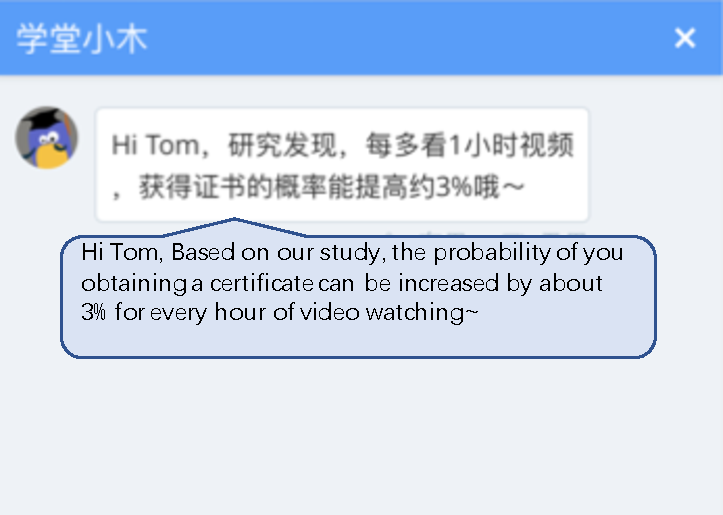
\includegraphics[height=3.7cm]{snapshot_1.pdf}
  	}
  	\subfigure[Strategy 2: Certificate driven in video]{
  		\centering
  		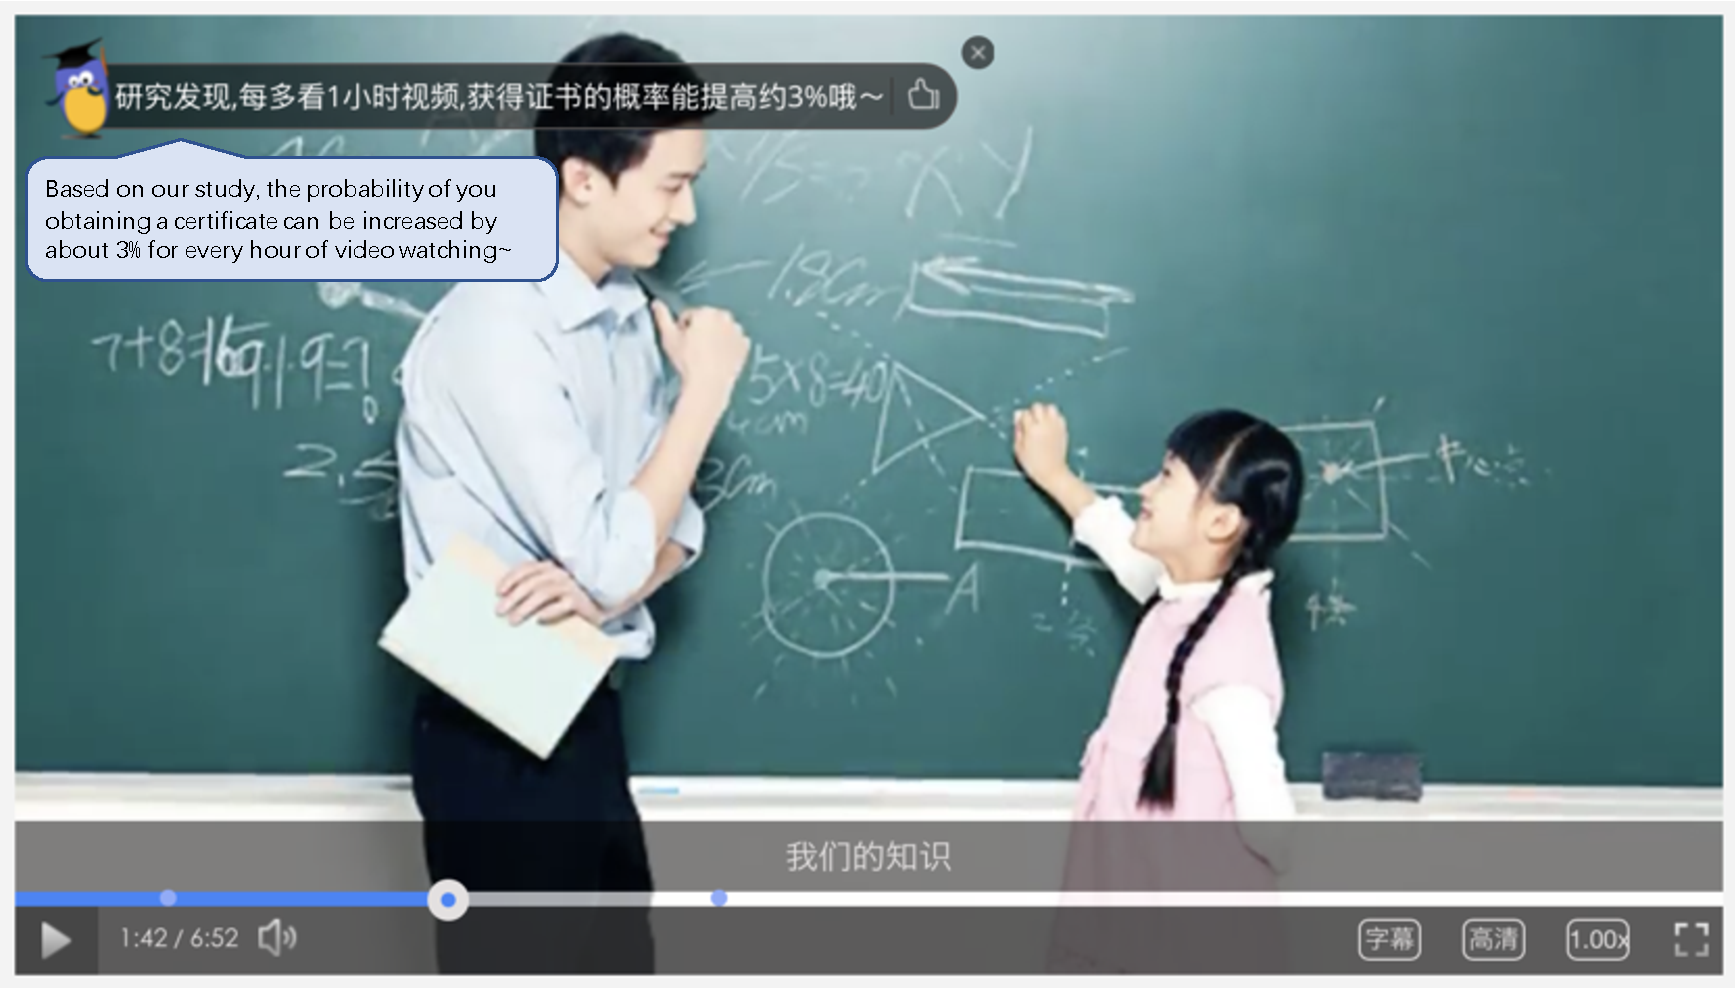
\includegraphics[height=3.7cm]{snapshot_2.pdf}
  	}
  	\subfigure[Strategy 3: Effort driven]{
  		\centering
  		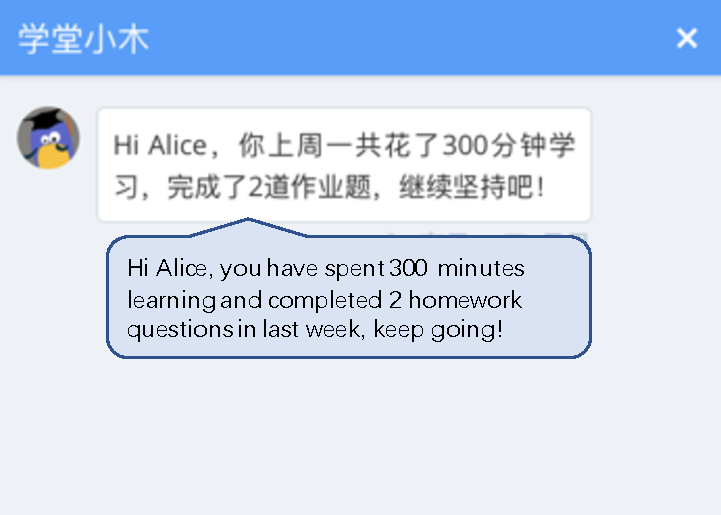
\includegraphics[height=3.7cm]{snapshot_new.pdf}
  	}
  	\caption{Snapshots of the three intervention strategies.} 
  	\label{fig:snapshot}
  \end{figure*}
  
  
  \subsection{Feature Contribution}
  	\begin{table}
		\caption{Contribution analysis for different engagements on KDDCUP dataset and IPM courses of XuetangX dataset.}
		\centering
		\setlength{\tabcolsep}{1.2mm}\begin{tabular}{lcccc}
		\hline \hline
			              & \multicolumn{2}{c}{KDDCUP} & \multicolumn{2}{c}{XuetangX} \\
			{Features}                &AUC (\%)   & F1 (\%)  & AUC (\%)   & F1 (\%)  \\ \hline 
			{All}                     & 90.07 & 92.27 & 86.50 & 90.95     \\ \hline
	   	  - Video         &  87.40 & 91.61     &84.40	  &90.32 \\ 
	      - Forum         & 88.61 & 91.93    & 85.13  &  90.41 \\
		  - Assignment   & 86.68  & 91.39     & 84.83  & 90.34 \\
		  %- (Video + Forum)       &  84.70 & 91.4      &84.42   & 90.31  \\
		  %- (Video + Assignment)   & 84.32& 91.17      &  83.14     &  89.63  \\
		  %- (Forum + Assignment)    & 85.07 &   91.49  &  84.72      & 90.29    \\
			 \hline \hline
 \end{tabular}

	  \label{tab:featImp}	
	\end{table}
	
	\begin{table}
    	\centering
    	\caption{Average attention weights of different clusters. C1-C5 --- Cluster 1 to 5; CAR --- average correct answer ratio. }
    	\small
    	\label{tab:AttnWeight}
    	\setlength{\tabcolsep}{1.8mm}\begin{tabular}{@{}c@{}|l@{}|c|c|c|c|c@{}}
    		\hline
    		\hline
    		Category &  Type   & C1& C2 & C3& C4&C5 \\
    		\hline
    		\multirow{3}{*}{video}&  \#watch &0.078 &0.060 &0.079&0.074 & 0.072\\	
    		\cline{2-7}
    		& \#stop     &0.090 & 0.055 & 0.092&0.092& 0.053\\
    		\cline{2-7}
    		& \#jump   &0.114 & 0.133 & 0.099&0.120& 0.125\\
    		\hline
    		\multirow{2}{*}{forum}&  \#question & 0.136 & 0.127 &0.138 & 0.139 & 0.129 \\
    		\cline{2-7}
    		& \#answer &0.142 &0.173&0.142&0.146&0.131\\
    		\hline
    		\multirow{2}{*}{assignment} & CAR &0.036 & 0.071 & 0.049& 0.049 & 0.122\\
    		\cline{2-7}
    		& \#reset  &0.159 & 0.157& 0.159& 0.125& 0.136\\
    		\hline
    		\multirow{2}{*}{session}    & seconds &0.146 &0.147& 0.138& 0.159& 0.151\\
    		\cline{2-7}                
    		&  count     &0.098 &0.075& 0.103&0.097& 0.081\\ 
    		\hline	
    		\hline
    	\end{tabular}
    	\normalsize
    \end{table}  
	
 	 In order to identify the importance of different kinds of engagement activities in this task, we conduct feature ablation experiments for three major activity features, i.e., video activity, assignment activity and forum activity, on two datasets. Specifically, we first input all the features to the \modelname{}, then remove every type of activity features one by one to watch the variety of performance. The results are shown in Table \ref{tab:featImp}. We can observe that all the three kinds of engagements are useful in this task. On KDDCUP, assignment plays the most important role, while on XuetangX, video seems more useful. 
 	 %Furthermore, the performance decrease rapidly when we remove the video activity and assignment activity together on XuetangX dataset.
 	 
 	 We also perform a fine-grained analysis for different features on different groups of users. Specifically, we feed a set of typical features into \modelname{}, and compute their average attention weights for each cluster. The results are shown in Table \ref{tab:AttnWeight}. We can observe that the distributions of attention weights on the five clusters are quite different. The most significant difference appears in CAR (correct answer ratio): Its attention weight on cluster 5 (hard workers) is much higher than those on other clusters, which indicates that correct answer ratio is most important in predicting dropout for hard workers. While for users with more forum activities (cluster 2), answering questions in forum seems to be the key factor, as the corresponding attention weight on ``\#question'' is the highest. Another interesting thing is about the users with high dropout rates (cluster 1, 3 and 4). They get much higher attention wights on the number of stopping video and watching video compared to cluster 2 and cluster 5. This indicates that the video activities play an more important role in predicting dropout for learners with poor engagements than active learners.
 	 
 	\hide{
	\subsection{Discussion for SPM Courses of XuetangX dataset}
	
		\begin{table}
		\centering
		\caption{Results on SPM courses }
		\setlength{\tabcolsep}{1mm}
        \begin{tabular}{ccccccc}
			\hline
			\hline
			Methods & LRC & SVM &RF &GBDT & \modelname{} & \modelname{}-en\\
			\hline
			AUC (\%) & 69.76 & 71.23 & 72.34 &72.21&73.47 & 74.11\\
			\hline
			\hline		
		\end{tabular}

		\label{tab:selfRes}
	\end{table}
	Besides experiments on IPM courses, we also conduct the same experiments on SPM courses of XuetangX  dataset. As shown in table \ref{tab:selfRes}, all the prediction results on SPM courses are rather lower than the results on IPM courses (table \ref{tab:allRes}). This is because SPM courses give more freedom to students, and do not require students to learn within a specified time. Therefore, there is more uncertainty for dropout prediction on SPM courses.
}

    %This is because of the big difference between this two kinds of courses: Instructor-paced courses follow a schedule that the instructor sets, assignments and exams of which have specific due dates. 
	
\begin{table}
		\centering
	\caption{Results of intervention by A/B test. WVT --- average time (s) of video watching; ASN --- average number of completed assignments; CAR --- average ratio of correct answers.} 
	\setlength{\tabcolsep}{0.7mm}
	\begin{tabular}{c|c|c|c|c}
		\hline
		\hline
	    Activity & No intervention & Strategy 1 & Strategy 2 &Strategy 3 \\
		\hline
		WVT & 4736.04 & 4774.59 & 5969.47 &3402.96\\
		\hline
	    ASN& 4.59 & 9.34* & 2.95 &11.19**\\
	    \hline
	    CAR & 0.29 & 0.34 & 0.22 &0.40\\
		\hline		
		\hline
	\end{tabular}
	*: $p-$value $\le 0.1$, **: $p-$value $\le 0.05$ by $t-$test.
	\label{tab:t-test}
\end{table}

	\subsection{From Prediction to Online Intervention}
	We have deployed the proposed algorithm onto \textit{XiaoMu}, an intelligent learning assistant subsystem on XuetangX, to help improve user retention. 
	 %For each course, we first provide online dropout prediction for all enrolled users. 
	 Specifically, we use our algorithm to predict the dropout probability of each user from a course.
	 If a user's dropout probability is greater than a threshold, 
	 \textit{XiaoMu} would send the user an intervention message.
	 %, trying to encourage her/him to learn on the courses. Specifically, 
	 We did an interesting A/B test by considering different strategies.
	 %consider three different intervention strategies:
	 \begin{itemize}
	 	 \item \textbf{Strategy 1: Certificate driven.} Users in this group will receive a message like \emph{``Based on our study, the probability of you obtaining a certificate can be increased by about 3\% for every hour of video watching.''}.% when user come to a course.
	 	 
	 	\item \textbf{Strategy 2: Certificate driven in video.} Users of this group will receive the same message as Strategy 1, but the scenario is 
	 	%Send user the same message as that of strategy 1 
	 	when the user is watching course video.
	 	
	 	\item \textbf{Strategy 3: Effort driven.} Users in group will receive a message to summarize her/his efforts used in this course such as
	 	%Send user a message of 
	 	\emph{``You have spent 300 minutes learning and completed 2 homework questions in last week, keep going!''}.% when user come to a course.
	 	\end{itemize}
 	
 	 	 	 Figure \ref{fig:snapshot} shows the system snapshots of three strategies. 
 	 	 	 We did the A/B test on four courses (i.e. Financial Analysis and Decision Making, Introduction to Psychology, C++ Programming and Java Programming) in order to examine the difference %effectiveness of 
 	 	 	 the different intervention strategies. Users %in these courses 
 	 	 	 are split into four groups, including three treatment groups corresponding to three intervention strategies and one control group. We collect two weeks of data and examine the video activities and assignment activities of different group of users. Table~\ref{tab:t-test} shows the results. 
 	 	 	 We see Strategy 1 and Strategy 3 can significantly improve users' engagement on assignment. Strategy 2 is more effective in encouraging users to watch videos.
 	 	 	 %We also did $t-$test results between the control group and each treatment group. 

	%We also  This strategy is based on our investigation for students' dropout reasons on XuetangX,  of which results indicate that over 20\% students drop out from XuetangX because no one remind them to learn on their enrolled courses.
		
     \section{Conclusion}
	In this paper, we conduct a systematical study for the dropout problem in MOOCs. We first conduct statistical analyses to identify factors that cause users' dropouts. We found several interesting phenomena such as dropout correlation between courses and dropout influence between friends.  
	%These observations are useful for teachers and MOOCs' designers to better navigate and design courses and platforms in the future. 
	Based on these analyses, 
we propose a context-aware feature interaction network (\modelname{}) to predict users' dropout probability. Our method achieves good performance on two datasets: KDDCUP and XuetangX.
The	proposed method has been deployed onto \textit{XiaoMu}, an intelligent learning assistant in XuetangX  to help improve students retention. We are also working on applying the method to several other systems such as ArnetMiner~\cite{Tang:08KDD}.
\hide{
\section{Acknowledgements}
Another author of this paper is Shuhuai Zhang, from PBC School of Finance, Tsinghua University.}


\vpara{Acknowledgements.}
The work is supported by the
%yuzhou li
National Natural Science Foundation of China (61631013),
the Center for Massive Online Education of Tsinghua University, and XuetangX. 
     
		
\bibliographystyle{IEEEtran}
	\bibliography{ref}
	
\end{document}
